% Indicate the main file. Must go at the beginning of the file.
% !TEX root = ../main.tex

%----------------------------------------------------------------------------------------
% CHAPTER TEMPLATE
%----------------------------------------------------------------------------------------


\chapter{Disseny del model} \label{disseny model} % Main chapter title

\label{Disseny del model} % Change X to a consecutive number; for referencing this chapter elsewhere, use \ref{ChapterX}
En aquest apartat s'expliquen totes les restriccions que conformen el model, des de la primera iteració del model, juntament amb les millores de comportament del model i les millores de rendiment aplicades. Per fer la lectura més còmoda els fragments de codi han estat alterats del llenguatge Python lleugerament en una mena de pseudocodi, a més també s'ha inclòs una versió simplificada de la formalització de cada restricció. La redacció de la formalització de les restriccions, contenen elements addicionals com per exemple \lstinline{ite(a,b,c)} per representar la funció if-then-else i també conté expressions com per exemple \lstinline{is_input(i, j)}, una funció que pot ser calculada en temps de compilació abans d'executar el procés de solving.

%----------------------------------------------------------------------------------------
% SECCIÓ 1: Implemenatció del model base
%----------------------------------------------------------------------------------------

\section{Implementació del model base}\label{model-base}

\subsection{Rutes}
Per implementar la noció de ruta s'ha usat la representació incremental on una casella que forma part d'una ruta ha de precedir una casella amb un valor de ruta inferior a ella i ser precedida per un element amb valor de ruta superior a ella. Per implementar aquesta representació s'ha creat una variable de tipus matriu \lstinline{route} de mida $width \times height$, el seu domini també és $[0..width * height]$, ja que una ruta pot ocupar com a màxim tota l'àrea del \textit{blueprint}, a banda també cal saber l'orientació dels elements que formen part de la ruta (inseridors i cintes) les quals es guarden en dues variables una per cada element \lstinline{conveyor} i \lstinline{inserter} aquestes de la mateixa manera que la ruta són matrius de mida $width \times height$ i el seu domini $[empty, north, east, south, west]$ on \textit{empty} significa que no hi ha cap inseridor o cinta present. Amb aquestes variables ja es poden definir les restriccions que conformen una ruta, principalment en són dues:

\begin{table}[h]
    \centering
    \begin{tabular}{|c|c|c|c|}
    \hline
    \textbf{Variable} & \textbf{Mida} & \textbf{Domini} & \textbf{Tipus} \\
    \hline
    route & $width \times height$ & $[0..width*height]$ & Int\\
    \hline
    inserter & $width \times height$ & $[empty, north, south, east, west]$ & EnumSort\\
    \hline
    conveyor & $width \times height$ & $[empty, north, south, east, west]$ & EnumSort\\
    \hline
    \end{tabular}
    \caption{Variables implicades a les rutes}
    \label{route-variables}
\end{table}

\subsubsection{Augment de ruta}
Aquesta restricció ens codifica qualsevol element que formi part d'una ruta, ha de tenir una casella adjacent la qual el seu valor de la ruta sigui superior. En aquest cas les caselles adjacents vàlides només són les que estan en la mateixa direcció que la cinta o inseridor corresponent a la posició de la ruta. A banda també s'ha de tenir en compte que les rutes poden acabar si a la posició de la ruta hi ha un inseridor i en la direcció on aquest apunta hi ha un assemblador. Per últim, una ruta també pot acabar si la posició de la ruta es tracta d'una casella output donada com a entrada del model. En aquests dos casos no cal assegurar que la posició en la direcció de l'inseridor el valor de ruta sigui més gran.\\
La restricció té la següent forma:
\begin{align*}
    &\forall i \in 0..width, \forall j \in 0..height \ such \ that: \lnot is\_output(i,j), \forall dir \in\{n, s, e, w\},\\
    &such \ that: (x,y)=pos(dir) \land \lnot outside(x+i, y+j).\\
    &\qquad (conveyor[i][j]=dir\rightarrow route[x+i][y+j]>route[i][j]) \ \land\\
    &\qquad ((inserter[i][j]=dir\land assembler[x+i][y+j]=0)\rightarrow \\
    &\qquad \qquad route[x+i][y+j]>route[i][j]) \ \land\\
    &\qquad ((inserter[i][j]=dir\land assembler[x+i][y+j]\neq0)\rightarrow(route[x+i][y+j]=0)
\end{align*}
On \lstinline{pos(dir)} és una funció que donada una direcció retorna el desplaçament relatiu a (0,0) que s'ha de fer per moure's en aquesta direcció. Per exemple \lstinline{pos(n)} = (-1,0), \lstinline{outside(x,y)} una funció que donada una posició retorna si aquesta està dins dels límits de la graella, \lstinline{is_output(i,j)} retorna si la posició és alguna de les caselles de sortida especificada a les entrades del model.
La implementació d'aquesta restricció es pot veure al codi de la figura \ref{code:forward_route}.

\begin{figure}
    \centering
    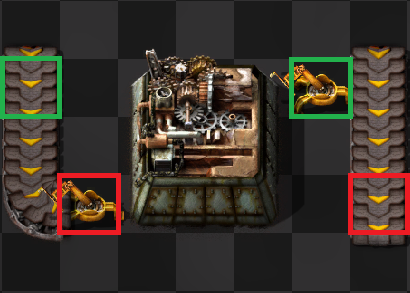
\includegraphics[width=0.5\linewidth]{Figures//captures_joc//exemples_model/start_end_pos.png}
    \caption{Possibles inicis ``verd'' i finals ``vermell" de rutes}
    \label{fig:start_end_route}
\end{figure}

\begin{lstlisting} [language=Python, caption=Forward Consistency, label=code:forward_route] 
for each cell (i, j) in the grid of size (height x width):
    if not is_output(i, j):
        inserter_output = []
        conveyor_output = []
        for each dir in [north, east, south, west]:
            x = i + displacement[dir][0]
            y = j + displacement[dir][1]
            if 0 <= x < height and 0 <= y < width:
                conveyor_output += Implies(conveyor[i][j] == dir,
                                      route[x][y] > route[i][j])
                                      
                inserter_output += If(And(inserter[i][j] == dir,
                                          assembler[x][y] == 0),
                                      route[x][y] > route[i][j])

                inserter_output += If(And(inserter[i][j] == dir,
                                          assembler[x][y] != 0),
                                      route[x][y] == 0)

            assert Implies(route[i][j] > 0, And(conveyor_output + inserter_output))
\end{lstlisting}

Cal mencionar que si les rutes només haguessin d'anar d'un punt A a un punt B amb aquesta restricció, seria suficient per assegurar que no es creïn cicles i que realment s'està creant una ruta que va del punt A al B, però com que en el nostre cas les rutes s'han de poder bifurcar, unir i arribar des de múltiples punts a múltiples punts, cal la següent restricció.

\subsubsection{Decrement de ruta}
Per poder incloure bifurcacions i unions ens cal una restricció que de manera similar a l'anterior restricció ens asseguri que si una cinta o inseridor forma part d'una ruta i no es tracta d'un inici de ruta, llavors cal que en una de les caselles veïnes, hi hagi un element de la ruta amb un valor inferior. Aquestes caselles veïnes seran diferents en funció de si l'element de la ruta tracta d'una cinta o un inseridor. Al cas de la cinta aquesta pot rebre input de qualsevol direcció que no sigui la mateixa que ella (Figura: \ref{fig:conveyor_in_out}) i en cas de l'inseridor aquest només pot rebre input de la casella en la direcció contrària a l'inseridor (Figura: \ref{fig:inserter_in_out}), a banda els inseridors també poder agafar objectes a un assemblador, així que en aquest cas forçarem que el valor de ruta a la posició de l'inseridor sigui 1 (inici de ruta).
Així doncs, la restricció queda de la següent manera:
\begin{align*}
    &\forall i \in 0..width, \forall j \in 0..height \ such \ that: \neg is\_input(i, j).\\
    &\qquad \bigvee_{dir \in \{n, s, e, w\}} \ such \ that: \ (x, y)=pos(dir) \land \neg outside(x+i, y+j).\\
    &\qquad \qquad ite\Big(conveyor[i][j]\neq dir\land conveyor[i][j]\neq empty,\\
    &\qquad \qquad \qquad route[x+i][y+j]<route[i][j]\land route[x+i][y+j]>0,false\Big)
\end{align*}
\begin{align*}
    &\forall i \in 0..width, \forall j \in 0..height \ such \ that: \neg is\_input(i,j), \forall dir \in \{n, s, e, w\},\\
    &such \ that: \ (x,y)=pos(dir) \land \neg outside(x+i,y+j).\\
    &\qquad ((inserter[i][j] = oppo(dir) \land assembler[x+i][y+j]=0) \rightarrow \\
    &\qquad \qquad (route[x+i][y+j]<route[i][j]\land route[x+i][y+j]>0)) \ \land \\
    &\qquad ((inserter[i][j] = oppo(dir) \land assembler[x+i][y+j]\neq0)\rightarrow route[i][j]=1)
\end{align*}
On la funció \lstinline{is_input(i, j)} retorna cert si la casella a la posició entrada tracta d'alguna de les caselles d'entrada especificades a les entrades del model, \lstinline{oppo(dir)} retorna la direcció oposada a la direcció entrada.
L'implemetació de la restricció es pot veure a la figura \ref{code:backwards_route}.

\begin{lstlisting}[language=Python, caption=Backwards Consistency, label=code:backwards_route]
for each cell (i, j) in the grid of size (height x width):
    if not is_input(i, j):
        inserter_input = []
        conveyor_input = []
        for each dir in [north, east, south, west]:
            x = i + displacement[dir][0]
            y = j + displacement[dir][1]
            if 0 <= x < height and 0 <= y < width:
                conveyor_input += If(And(conveyor[i][j] != dir,
                                         conveyor[i][j] != empty),
                                     And(route[x][y] < route[i][j],
                                         route[x][y] > 0),
                                     False)
        
                inserter_input += Implies(
                                    And(inserter[i][j] == opposite(dir),
                                        assembler[x][y] == 0),
                                    And(route[x][y] < route[i][j],
                                        route[x][y] > 0))
        
                inserter_input += Implies(
                                    And(inserter[i][j] == opposite(dir),
                                        assembler[x][y] != 0),
                                    route[i][j] == 1)

    assert Implies(inserter[i][j] != empty, And(inserter_input))
    assert Implies(conveyor[i][j] != empty, Or(conveyor_input))
\end{lstlisting}

Amb aquestes dues restriccions assegurem que la ruta no generi bucles i arribi als punts corresponents, però no ens assegura que l'orientació dels elements ni quins elements poden estar interconnectats entre si, així doncs per acabar de definit una ruta cal afegir quines entrades i sortides són vàlides per una cinta i un inseridor:

\subsubsection{Entrada i sortida de les cintes}
Amb aquestes dues restriccions definim quines entrades i sortides són vàlides per una cinta. Pel que fa a les entrades pot rebre objectes per qualsevol de les posicions adjacents que no estiguin en la mateixa direcció que la mateixa cinta, a més aquestes caselles poden ser tant inseridors com cintes. A més la cinta o inseridor que estigui a la casella veïna ha d'apuntar a la cinta, és a dir, la seva direcció pot ser qualsevol menys l'oposada a la cinta. La restricció queda així:
\begin{align*}
    & \forall i \in 0..width, \forall j \in 0..height \ such \ that: \neg is\_input(i, j). \\
    & \qquad conveyor[i][j]\neq empty \rightarrow\\
    & \qquad \qquad \bigvee_{dir \in \{n, s, e, w\}} such \ that: \ (x, y)=pos(dir) \land \neg outside(x+i, y+j).\\
    & \qquad \qquad \qquad ite\Big(conveyor[i][j]\neq dir,\\
    & \qquad \qquad \qquad \qquad conveyor[x+i][y+j]=oppo(dir) \ \lor \\ 
    & \qquad \qquad \qquad \qquad inserter[x+i][y+j]=oppo(dir),\\
    & \qquad \qquad \qquad \qquad false\Big)
\end{align*}
La implementació es pot veure a la figura \ref{code:conv_input}.

\begin{lstlisting}[language=Python, caption=Conveyor Input, label=code:conv_input]
for each cell (i, j) in the grid of size (height x width):
    if not is_input(i, j):
        direction_clauses = []
        for each dir in [north, east, south, west]:
            x = i + displacement[dir][0]
            y = j + displacement[dir][1]
            if 0 <= x < height and 0 <= y < width:
                direction_clauses += 
                    If(conveyor[i][j] != dir,
                        Or(conveyor[x][y] == opposite(dir),
                            inserter[x][y] == opposite(dir)),
                        False))
        assert Implies(conveyor[i][j] != empty, Or(direction_clauses))
\end{lstlisting}


D'altra banda, una cinta només pot treure elements per la casella adjacent a la direcció a la qual apunta, aquesta casella veïna només pot estar ocupada per una cinta o un \textit{insrter}, la direcció de la qual ha de ser qualsevol menys l'oposada a la cinta. La restricció queda de la següent manera:
\begin{align*}
    & \forall i \in 0..width \ \forall j \in 0..height \ such \ that: \neg is\_output(i, j). \\
    & \qquad \bigvee_{dir \in \{n, s, e, w\}} such \ that: \ (x, y)=pos(dir) \land \neg outside(x+i, y+j).\\
    & \qquad \qquad ite\Big(conveyor[i][j]=dir, \\
    & \qquad \qquad \qquad (conveyor[x+i][y+j] \neq empty \land conveyor[x+i][y+j] \neq oppo(dir))\\
    & \qquad \qquad \qquad \lor inserter[x+i][y+j]=dir,false\Big)
\end{align*}
La implementació es pot veure a la figura \ref{code:conv_output}.
\begin{lstlisting}[language=Python, caption=Conveyor Output, label=code:conv_output]
for each cell (i, j) in the grid of size (height x width):
    if not is_output(i, j):
        direction_clauses = []
        for each dir in [north, east, south, west]:
            x = i + displacement[dir][0]
            y = j + displacement[dir][1]
            if 0 <= x < height and 0 <= y < width:
                direction_clauses += 
                    If(
                        conveyor[i][j] == dir,
                        Or(
                            And(conveyor[x][y] != empty,
                                conveyor[x][y] != opposite(dir)),
                            inserter[x][y] == dir),
                        False)
        assert Implies(conveyor[i][j] != empty, Or(direction_clauses))
\end{lstlisting}

\subsubsection{Entrada i sortida dels inseridors}
Els inseridors són molt similars a les cintes a l'hora de rebre objectes, però amb dues particularitats, primer només poden rebre objectes de la casella adjacent en la direcció contrària a l'inseridor i segon, aquesta casella adjacent també pot ser un assemblador. A l'hora de treure objectes de la mateixa manera que les cintes, només ho pot fer en la casella adjacent que es troba en la mateixa direcció, però en aquesta casella només hi pot haver una cinta que no apunti en la direcció oposada a l'inseridor o bé un assemblador. Les restriccions són les següents:
\begin{align*}
    & \forall i \in 0..width, \forall j \in 0..height \ \neg is\_input(i, j).\\
    & \qquad \bigvee_{dir \in \{n, s, e, w\}}such \ that: \ (x, y)=pos(dir) \land \neg outside(x+i, y+j) \ \land\\
    & \qquad \neg is\_input(x+i, y+j).\\
    & \qquad \qquad ite\Big(inserter[i][j]=oppo(dir),\\
    & \qquad \qquad \qquad conveyor[x+i][y+j]\neq empty \lor assembler[x+i][y+j]\neq 0, false\Big)
\end{align*}
Amb implementació a \ref{code:inserter_input}.

\begin{align*}
    & \forall i \in 0..width \ \forall j \in 0..height \ \neg is\_output(i, j),\\
    & \qquad \bigvee_{dir \in \{n, s, e, w\}} such \ that: \ (x, y)=pos(dir) \land \neg outside(x+i, y+j)\\
    & \qquad \qquad ite\Big(inserter[i][j]=dir,\\
    & \qquad \qquad \qquad (conveyor[x+i][y+j]\neq empty \land conveyor[x+i][y+j]\neq oppo(dir)) \lor\\
    & \qquad \qquad \qquad assembler[x+i][y+j]\neq 0,false\Big)
\end{align*}
Implementada a \ref{code:inserter_output}.
\begin{lstlisting}[language=Python, caption=Inserter Input, label=code:inserter_input]
for each cell (i, j) in the grid of size (height x width):
    if not is_input(i, j):
        direction_clauses = []
        for each dir in [north, east, south, west]:
            x = i + displacement[dir][0]
            y = j + displacement[dir][1]
            if 0 <= x < height and 0 <= y < width:
                if not is_output(x, y):
                    direction_clauses += 
                        If(inserter[i][j] == opposite(dir),
                            Or(conveyor[x][y] != empty,
                                assembler[x][y] != 0),
                            False)
        assert Implies(inserter[i][j] != empty, Or(direction_clauses))
\end{lstlisting}

\begin{lstlisting}[language=Python, caption=Inserter Output, label=code:inserter_output]
for each cell (i, j) in the grid of size (height x width):
    if not is_output(i, j):
        direction_clauses = []
        for each dir in [north, east, south, west]:
            x = i + displacement[dir][0]
            y = j + displacement[dir][1]
            if 0 <= x < height and 0 <= y < width:
                direction_clauses += 
                    If(inserter[i][j] == dir,
                        Or(And(conveyor[x][y] != empty,
                                conveyor[x][y] != opposite(dir)),
                            assembler[x][y] != 0),
                        False)
        assert Implies(inserter[i][j] != empty, Or(direction_clauses))
\end{lstlisting}

Amb totes aquestes restriccions ja queden definides les rutes, tot seguit alguns exemples senzills a les figures \ref{fig:route_ex1}, \ref{fig:route_ex2} i l'assignació de les variables \lstinline{route}, \lstinline{inserter} i \lstinline{conveyor} de l'exemple \ref{fig:solucio_exemple} a la figura \ref{fig:route_ex_real}\\


\begin{figure}[H]
    \centering
    \begin{subfigure}{.45\textwidth}
        \centering
        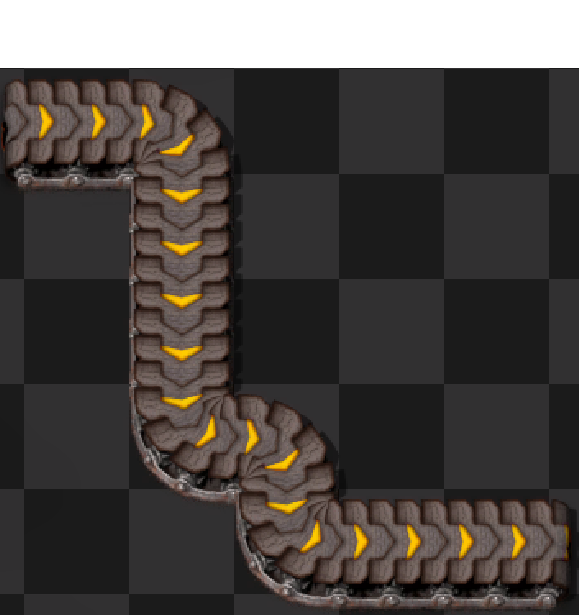
\includegraphics[width=0.9\linewidth]{Figures/captures_joc/exemples_model/5x5_route_instance.png}
        \caption{Representació gràfica de la variable \lstinline{conveyor}}
    \end{subfigure}
    \hspace{1cm}
    \begin{subfigure}{.45\textwidth}
        \centering
        \newcolumntype{C}[1]{>{\centering\arraybackslash}m{#1}}
        \renewcommand{\arraystretch}{2.5} % Adjust the row height
        \begin{tabular}{|C{1cm}|C{1cm}|C{1cm}|C{1cm}|C{1cm}|}
            \hline
            1 & 6 & 0 & 0 & 0\\ \hline
            0 & 8 & 0 & 0 & 0\\ \hline
            0 & 13 & 0 & 0 & 0\\ \hline
            0 & 18 & 19 & 0 & 0\\ \hline
            0 & 0 & 21 & 22 & 23\\ \hline
        \end{tabular}
        \caption{Assignacions de la variable \lstinline{route}}
    \end{subfigure}
    \caption{Exemple bàsic d'assignacions que compleixen amb les restriccions que defineixen una ruta}
    \label{fig:route_ex1}
\end{figure}



\begin{figure}[H]
    \centering
    \begin{subfigure}{.45\textwidth}
        \centering
        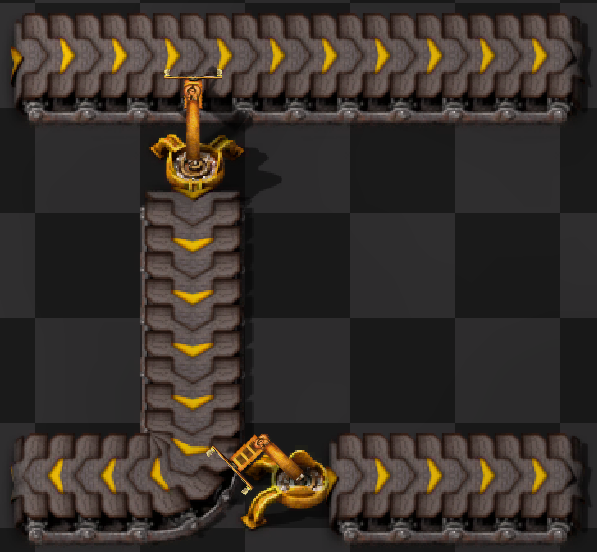
\includegraphics[width=0.9\linewidth]{Figures/captures_joc/exemples_model/5x5_instance_3_out.png}
        \caption{Representació gràfica de la variable \lstinline{conveyor}}
    \end{subfigure}
    \hspace{1cm}
    \begin{subfigure}{.45\textwidth}
        \centering
        \newcolumntype{C}[1]{>{\centering\arraybackslash}m{#1}}
        \renewcommand{\arraystretch}{2.5} % Adjust the row height
        \begin{tabular}{|C{1cm}|C{1cm}|C{1cm}|C{1cm}|C{1cm}|}
            \hline
            1 & 2 & 22 & 23 & 24\\ \hline
            0 & 3 & 0 & 0 & 0\\ \hline
            0 & 4 & 0 & 0 & 0\\ \hline
            0 & 7 & 0 & 0 & 0\\ \hline
            14 & 12 & 15 & 20 & 23\\ \hline
        \end{tabular}
        \caption{Assignacions de la variable \lstinline{route}}
    \end{subfigure}
    \caption{Exemple d'assignacions que compleixen amb les restriccions que defineixen una ruta, aquesta amb bifurcacions}
    \label{fig:route_ex2}
\end{figure}

\begin{figure}[h]
    \centering
    \begin{subfigure}{0.45\textwidth}
        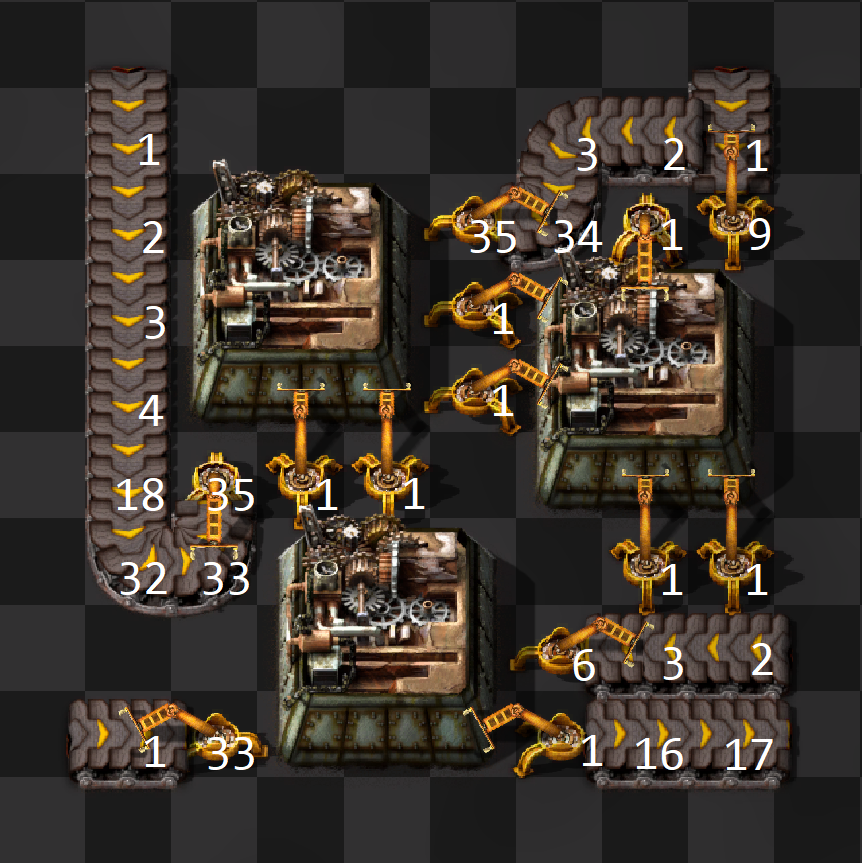
\includegraphics[width=\textwidth]{Figures/captures_joc/exemples_model/example_route_values.png}
        \caption{Variable \textit{route}}
    \end{subfigure}
    \hfill
    \begin{subfigure}{0.45\textwidth}
        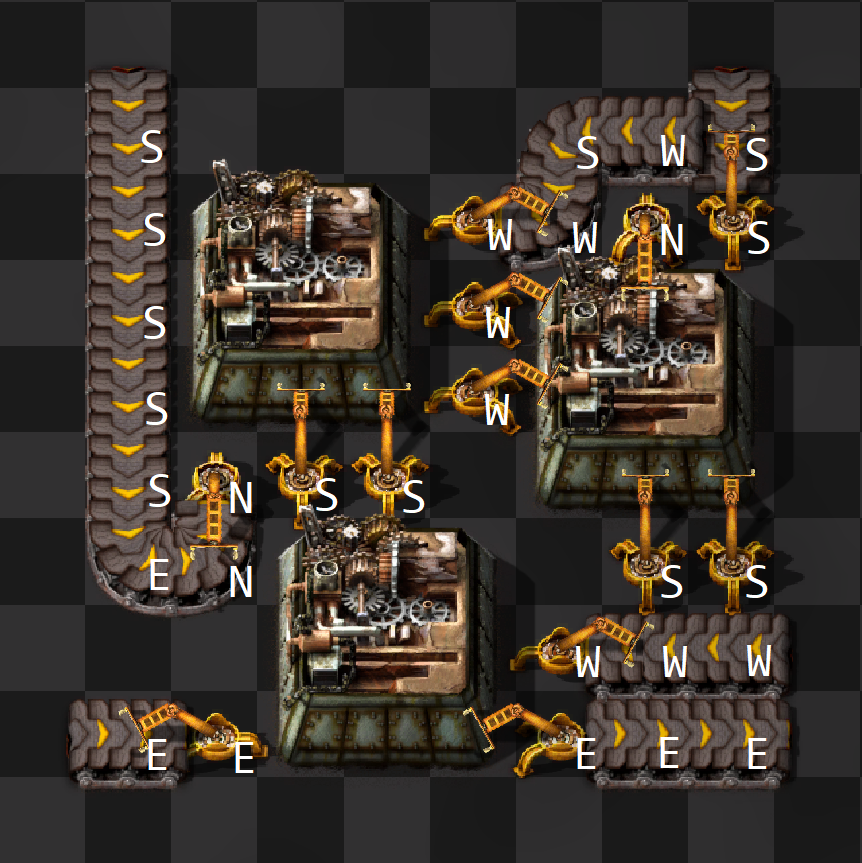
\includegraphics[width=\textwidth]{Figures/captures_joc/exemples_model/example_dir_values.png}
        \caption{Variable inseridor i cinta}
    \end{subfigure}
    \caption{Assignacions de les variables a l'exemple, les assignacions amb valor 0 o \textit{empty} s'han ignorat, les direccions de l'inseridor i \textit{conveyor} s'han posat en comú.}
    \label{fig:route_ex_real}
\end{figure}



\subsection{Restriccions dels assembladors}
A l'hora de representar els assembladors hem de tenir en compte que ocupen un espai de 3x3 caselles, això complica la detecció de col·lisions entre ells i entre la resta d'objectes, així doncs, s'han usat dues variables per poder tenir control sobre la posició i àrea que ocupa cada assemblador. La primera variable \lstinline{assembler} guarda la posició del centre de l'assemblador i tracta d'una matriu de mida $width-2 \times height-2$ amb domini $[0..(width/3)*(height/3)]$. El motiu pel qual la mida de la matriu no és la del \textit{blueprint} és perquè els assembladors en ocupar 3x3 caselles sabem que no hi ha cap assignació al perímetre exterior que sigui vàlida, així que ignorem aquestes posicions. La segona variable \lstinline{collision_area} és una matriu de mida $width \times height$ i domini $[0..(width/3)*(height/3)]$. Aquesta variable guarda en quines posicions hi ha un assemblador, tot seguit les restriccions que es creen amb aquestes variables que ens permeten el control sobre les col·lisions entre assembladors, a més també serveixen per a restriccions futures saber exactament on hi ha un assemblador.

\begin{table}[h]
    \centering
    \small
    \begin{tabular}{|c|c|c|c|}
    \hline
    \textbf{Variable} & \textbf{Mida} & \textbf{Domini} & \textbf{Tipus}\\
    \hline
    assembler & $(width-2) \times (height-2)$ & $[0..(width/3)*(height/3)]$ & Int\\
    \hline
    collision\_area & $width \times height$ & $[0..(width/3)*(height/3)]$ & Int\\
    \hline
    \end{tabular}
    \caption{Variables implicades als assembladors}
    \label{assembler-variables}
\end{table}

\subsubsection{Col·lisió dels assembladors}
Aquesta restricció s'assegura que per cada posició de la matriu de la variable \lstinline{assembler} on el valor sigui superior a 0 (és a dir que hi ha un assemblador), les 3x3 caselles adjacents a la matriu de la variable \lstinline{collision_area} hagin de ser del mateix valor. D'aquesta manera ja tenim una variable on tenim representades les caselles on hi ha assembladors.
Amb aquesta restricció ja ens assegurem que no hi hagi col·lisions entre assembladors, ja que en cas que el \textit{solver} hagi assignat dos assembladors a posicions on intersequen, aquesta restricció farà que hi hagi caselles que han de prendre dos valors diferents, avaluant així a fals i sent necessari la reubicació de les posicions per evitar-ho.
\begin{align*}
    &\forall i \in 0..width-2, \forall j \in 0..height-2.\\
    &\qquad assembler[i][j]\neq0 \rightarrow\\
    &\qquad \qquad \bigwedge_{(x, y) \in neigh\_pos() \ such \ that: \neg outside(x+i+1, y+j+1)}.\\
    &\qquad \qquad \qquad collision\_area[x+i+1][y+j+1]=assembler[i][j]
\end{align*}
On la funció \lstinline{neigh_pos()}, retorna totes les posicions adjacents a una casella centrada a (0,0), concretament [(-1,-1),(-1,0),(-1,1),(0,1),(1,1),(1,0),(1,-1),(0,-1)].
La restricció s'implementa a \ref{code:assembler_collision}.

\begin{lstlisting}[language=Python, caption=Assembler Collision, label=code:assembler_collision]
for each cell (i, j) in the grid of size (height-2 x width-2):
    surround_collision = []
    for each neighbor (di, dj) in the 3x3 grid centered at (i, j):
        x = di + i + 1
        y = dj + j + 1
        if 0 <= x < height and 0 <= y < width:
            surround_collision += collision_area[x][y] == assembler[i][j]
    assert Implies(assembler[i][j] != 0, And(surround_collision))
\end{lstlisting}


Per assegurar que no hi hagi col·lisions entre assembladors, aquesta restricció és suficient. Així i tot, si volem usar la variable \lstinline{assembler_collision} per saber exactament on hi ha un assemblador per a futures restriccions que impliquen als inseridors, amb això no n'hi ha prou, ja que no estem forçant a les caselles on no hi ha assembladors que prenguin el valor 0.

\begin{figure}[H]
    \centering
    \begin{subfigure}{.45\textwidth}
        \centering
        \newcolumntype{C}[1]{>{\centering\arraybackslash}m{#1}}
        \renewcommand{\arraystretch}{2.5} % Adjust the row height
        \begin{tabular}{|C{1cm}|C{1cm}|C{1cm}|}
            \hline
            0 & 0 & 0\\ \hline
            0 & 0 & 0\\ \hline
            0 & 0 & 0\\ \hline
        \end{tabular}
        \caption{Variable \lstinline{assembler} sense cap assemblador present}
    \end{subfigure}
    \hspace{1cm}
    \begin{subfigure}{.45\textwidth}
        \centering
        \newcolumntype{C}[1]{>{\centering\arraybackslash}m{#1}}
        \renewcommand{\arraystretch}{2.5} % Adjust the row height
        \begin{tabular}{|C{1cm}|C{1cm}|C{1cm}|C{1cm}|C{1cm}|}
            \hline
            0 & 0 & 0 & 0 & 0\\ \hline
            0 & 1 & 1 & 0 & 0\\ \hline
            1 & 0 & 0 & 0 & 0\\ \hline
            1 & 1 & 0 & 1 & 0\\ \hline
            0 & 0 & 1 & 0 & 0\\ \hline
        \end{tabular}
        \caption{Variable \lstinline{collision_area} prenent valors $>$ 0 on no hi ha assembladors}
    \end{subfigure}
    \caption{Exemple de com hi ha assignacions vàlides que no representen les posicions on es troben els assembladors}
\end{figure}


\subsubsection{Enllaçar col·lisió amb assemblador}
Amb aquesta restricció hem d'aconseguir que \lstinline{collision_area} només pregui valors $>$ 0 on hi ha un assemblador, per a fer-ho només cal assegurar que per cada posició de la matriu de la variable \lstinline{collision_area} si hi ha una casella que ha pres valor $>$ 0 llavors una de les 8 caselles adjacents a la variable \lstinline{assembler} ha de tenir un valor $>$ 0.

\begin{figure}[H]
    \centering
    \begin{subfigure}{.45\textwidth}
        \centering
        \newcolumntype{C}[1]{>{\centering\arraybackslash}m{#1}}
        \renewcommand{\arraystretch}{1.5} % Adjust the row height
        \begin{tabular}{|C{0.5cm}|C{0.5cm}|C{0.5cm}|C{0.5cm}|C{0.5cm}|C{0.5cm}|}
            \hline
            0 & 0 & 0 & 0 & 0 & 0\\ \hline
            0 & 0 & 0 & 0 & 0 & 0\\ \hline
            0 & 0 & 0 & 0 & 0 & 0\\ \hline
            0 & 1 & 0 & 0 & 0 & 4\\ \hline
            0 & 0 & 0 & 0 & 0 & 0\\ \hline
            0 & 0 & 0 & 0 & 0 & 0\\ \hline
        \end{tabular}
        \caption{Variable \lstinline{assembler} amb 2 assignacions $>$ 0}
    \end{subfigure}
    \hspace{1cm}
    \begin{subfigure}{.45\textwidth}
        \centering
        \newcolumntype{C}[1]{>{\centering\arraybackslash}m{#1}}
        \renewcommand{\arraystretch}{1.5} % Adjust the row height
        \begin{tabular}{|C{0.5cm}|C{0.5cm}|C{0.5cm}|C{0.5cm}|C{0.5cm}|C{0.5cm}|C{0.5cm}|C{0.5cm}|}
            \hline
            0 & 0 & 0 & 0 & 0 & 0 & 0 & 0\\ \hline
            0 & 0 & 0 & 0 & 0 & 0 & 0 & 0\\ \hline
            0 & 0 & 0 & 0 & 0 & 0 & 0 & 0\\ \hline
            0 & 1 & 1 & 1 & 0 & 4 & 4 & 4\\ \hline
            0 & 1 & 1 & 1 & 0 & 4 & 4 & 4\\ \hline
            0 & 1 & 1 & 1 & 0 & 4 & 4 & 4\\ \hline
            0 & 0 & 0 & 0 & 0 & 0 & 0 & 0\\ \hline
            0 & 0 & 0 & 0 & 0 & 0 & 0 & 0\\ \hline
        \end{tabular}
        \caption{\lstinline{collision_area} prenent valors només a l'àrea 3x3 on hi ha presents assembladors}
    \end{subfigure}
    \caption{Exemple de com amb l'anterior restricció s'aconsegueix representar exactament la col·lisió dels assembladors}
\end{figure}

\begin{align*}
    & \forall i \in 0..width, \forall j \in 0..height. \\
    & \qquad collision\_area[i][j]\neq0 \rightarrow \\
    & \qquad \qquad  \bigvee_{(x, y) \in neigh\_pos() \ such \ that: \neg outside(x+i-1, y+j-1)}.\\
    & \qquad \qquad \qquad collision\_area[x+i-1][y+j-1] = assembler[i][j]
\end{align*}
Implementada a \ref{code:assembler_link}.

\begin{lstlisting}[language=Python, caption=Link Assembler Collision, label=code:assembler_link]
for each cell (i, j) in the grid of size (height x width):
    neighbors = []
    for each neighbor (di, dj) in the 3x3 grid centered at (i, j):
        x = di + i - 1
        y = dj + j - 1
        if 0 <= x < placement_height and 0 <= y < placement_width:
            neighbors += assembler[x][y] == collision_area[i][j]
    assert Implies(collision_area[i][j] != 0,
              Or(neighbors))
\end{lstlisting}

\subsection{Tipus d'objectes}
Per modelar quin tipus d'objecte transporta cada casella s'ha usat la variable \lstinline{item_flow} que tracta d'una matriu de mida $width \times height$ amb domini $[0..max\_items]$. \lstinline{max_items} és un upper bound que es pot calcular a partir de les entrades del model, concretament donat l'ítem de sortida que el \textit{blueprint} ha de produir, podem analitzar quines receptes el produeixen i quins elements requereixen aquestes receptes així recursivament fins que només quedin objectes bàsics que no s'obtenen com a sortida d'una recepta.\\
Les restriccions associades al flux d'objectes són les següents:
\begin{table}[h]
    \centering
    \begin{tabular}{|c|c|c|c|}
    \hline
    \textbf{Variable} & \textbf{Mida} & \textbf{Domini} & \textbf{Tipus}\\
    \hline
    item\_flow & $width \times height$ & $[0..max\_items]$ & Int\\
    \hline
    \end{tabular}
    \caption{Variables implicades al tipus d'objectes}
    \label{item_flow-variables}
\end{table}

\subsubsection{Forma part de la ruta} \label{subsubsec:part_of_route_object_type}
Amb aquesta restricció fem que per totes les posicions \lstinline{(i, j)} de la variable \lstinline{route} que prenguin un valor superior a 0, és a dir que formen part d'una ruta, forcen que a la mateixa posició \lstinline{(i, j)} de la variable \lstinline{item_flow} el valor pres sigui superior a 0, és a dir que transporten algun objecte.
\begin{align*}
    &\forall i \in 0..width, \forall j \in 0..height.\\
    &\qquad route[i][j]>0 \leftrightarrow item\_flow[i][j]>0
\end{align*}
L'implementació de la restricció es troba a \ref{code:part_of_route_item_flow}
\begin{lstlisting}[language=Python, caption=Part of Route, label=code:part_of_route_item_flow]
for each cell (i, j) in the grid of size (height x width):
        assert (route[i][j] > 0) == (item_flow[i][j] > 0)
\end{lstlisting}

\subsubsection{Entrada i sortida d'objectes}
Com s'ha comentat a l'apartat \nameref{sec:blueprint_problem} una de les entrades del model tracta d'especificar quins objectes hi ha d'haver a les caselles d'entrada i sortida. Aquesta restricció, doncs, s'encarrega d'assegurar que aquestes caselles portin els objectes especificats.
\begin{align*}
    &\forall (i, j) \in input\_cells().\\
    &\qquad item\_flow[i][j] = input\_item(i, j)
\end{align*}
\begin{align*}
    &\forall (i, j) \in output\_cells().\\
    &\qquad item\_flow[i][j] = output\_item(i, j)
\end{align*}
Les funcions \lstinline{input_cells()} i \lstinline{output_cells()} retornen una llista de posicions que indiquen les caselles d'entrada i sortida, entrades al model. A més les funcions \lstinline{input_item(i,j)} i \lstinline{output_item(i,j)}, retornen l'objecte que hi ha a la casella d'entrada i sortida respectivament.
Les restriccions queden implementades a \ref{code:input_output_items}
\begin{lstlisting}[language=Python, caption=Item Input i Output, label=code:input_output_items]
for each cell (i, j) in input_cells:
    assert item_flow[i][j] == input_item(i, j)

for each cell (i, j) in output_cells:
    assert item_flow[i][j] == output_item(i, j)
\end{lstlisting}

\subsubsection{Propagació del tipus d'objectes}
Finalment, la restricció més important és la que s'encarrega d'assegurar que els objectes especificats a les entrades, sortides i els objectes requerits i produïts per les receptes associades als assembladors, es distribueixen correctament per les rutes.\\
Per aconseguir aquest comportament el que s'ha fet és, per totes les posicions del \textit{blueprint}, i cada posició ortogonalment veïna a la casella que estigui dins el \textit{blueprint}, si la casella té un valor a la variable \lstinline{route} > 0, la direcció on es troba respecte a la direcció de la casella central és l'oposada i la casella central tracta d'un inseridor, llavors el valor de la variable \lstinline{item_flow} a la posició de l'inseridor ha de ser la mateixa que la de la posició veïna.\\
D'altra banda, i de manera molt similar si la casella ortogonalment veïna té un valor a la variable \lstinline{route} > 0 i es troba en la mateixa direcció que l'inseridor central llavors és la casella veïna que ha de tenir el mateix valor a \lstinline{item_flow} que la casella central.\\
Finalment, si la casella central tracta d'una cinta, només cal assegurar que la casella veïna que es troba en la mateixa direcció que la cinta central ha de tenir el mateix valor a \lstinline{item_flow} que la cinta.\\
\begin{align*}
    &\forall i \in 0..width, \forall j \in 0..height \ such \ that: \neg is\_input(i,j), \forall dir \in \{n, s, e, w\},\\
    &such \ that: \ (x,y)=pos(dir) \land \neg outside(x+i, y+j).\\
    &\qquad ((inserter[i][j] = oppo(dir) \land  route[x+i][y+j] > 0) \rightarrow\\
    &\qquad \qquad item\_flow[i][j] = item\_flow[x+i][y+j]) \ \land \\
    &\qquad ((inserter[i][j] = dir \land route[x+i][y+j] > 0) \rightarrow\\
    &\qquad \qquad item\_flow[x+i][y+j] = item\_flow[i][j])
\end{align*}

\begin{align*}
    &\forall i \in 0..width, \forall j \in 0..height \ such \ that: \neg is\_output(i,j), \forall dir \in \{n, s, e, w\},\\
    &such \ that: \ (x,y)=pos(dir) \land \neg outside(x+i, y+j).\\
    &\qquad conveyor[i][j] = dir \rightarrow item\_flow[i][j] = item\_flow[x+i][y+j]
\end{align*}

La implementació d'aquestes restriccions es pot veure a \ref{code:item_carry}.

\begin{lstlisting}[language=Python, caption=Item Carry, label=code:item_carry]
for each cell (i, j) in the grid of size (height x width):
    inserter_carry = []
    conveyor_carry = []
    for each dir in [north, east, south, west]:
        x = i + displacement[dir][0]
        y = j + displacement[dir][1]
        if 0 <= x < height and 0 <= y < width:
            if not is_input(i, j):
                inserter_carry += 
                    Implies(And(inserter[i][j] == opposite(dir),
                                route[x][y] > 0),
                            item_flow[i][j] == item_flow[x][y])
                inserter_carry += 
                    Implies(And(inserter[i][j] == dir,
                                route[x][y] > 0),
                            item_flow[x][y] == item_flow[i][j])
            if not is_output(i, j):
                conveyor_carry += 
                    Implies(conveyor[i][j] == dir,
                            item_flow[x][y] == item_flow[i][j])

    assert Implies(inserter[i][j] != empty, And(inserter_carry))
    assert Implies(conveyor[i][j] != empty, And(conveyor_carry))
\end{lstlisting}

Alguns detalls importants sobre la restricció són:\\
Només cal tenir en compte que la casella veïna tingui un valor a la variable \lstinline{route} més gran que zero \\ si la casella central tracta d'un inseridor, ja que són els únics elements d'una ruta que a la seva entrada o sortida hi pot haver un assemblador és a dir una posició on mai hi pot haver un valor d'\lstinline{route} més gran que zero.\\

Les caselles de sortida del \textit{blueprint}, que només poden ser cintes, no han de propagar el seu objecte, d'aquí la comprovació de \lstinline{if not is_output(i, j)}.\\

Tot i que no hi pot haver inseridors a les posicions d'entrada d'objectes, s'ha afegit la comprovació de \lstinline{if not is_input(i, j)}, ja que ens estalvia afegir restriccions addicionals.\\

Les implicacions finals són redundants, ja que només iterem per les direccions \lstinline{[north, east, south, west]} i les implicacions anteriors asseguren que les direccions de les cintes i inseridors siguin la mateixa que iterem o l'oposada, les quals mai seran \lstinline{empty}, així i tot, les implicacions finals ajuden a reduir el temps de solving, d'alguna manera deuen estar ajudant al solver a propagar més fàcilment les implicacions anteriors.

\subsection{Quantitat d'objectes}
Per determinar la quantitat d'objectes que passen per una casella, he decidit usar la mesura d'objectes per minut, el motiu és perquè té un bon balanç entre precisió i eficiència a l'hora de definir el domini de la variable.\\
Modelar aquesta mecànica del joc és de les més costoses i difícils de replicar, tot seguit explico les variables usades, el raonament els pros i contres.\\
Per cada casella cal saber quants objectes entren i quants surten, per poder modelar aquests objectes se sumen i reparteixen. Així doncs, s'han usat dues variables: \lstinline{input_flow_rate} i \lstinline{output_flow_rate} que són dues matrius de mida $width \times height$ i els seus dominis $[0..450]$ on 450 és el màxim nombre d'objectes per minut que un element de la ruta pot dur, en aquest cas la cinta, així que s'haurà d'anar amb compte i assegurar que els inseridors no duguin més objectes per minut que la seva capacitat màxima de 50.\\
Les variables \lstinline{output_flow_rate} i \lstinline{input_flow_rate} són de tipus real, ja que les ràtios d'entrada/sortida de moltes receptes fan que una entrada entera d'objectes minut produeixi un nombre decimal d'objectes de sortida, i arrodonir aquests representa perdre molta precisió i allunyar-se dels casos reals que es podrien assolir amb les mecàniques originals del joc.

Les restriccions associades a aquestes variables que modelen la quantitat d'objectes que circulen pel \textit{blueprint} són les següents:
\begin{table}[h]
    \centering
    \begin{tabular}{|c|c|c|c|}
    \hline
    \textbf{Variable} & \textbf{Mida} & \textbf{Domini} & \textbf{Tipus}\\
    \hline
    input\_flow\_rate & $width \times height$ & $[0..450]$ & Real\\
    \hline
    output\_flow\_rate & $width \times height$ & $[0..450]$ & Real\\
    \hline
    \end{tabular}
    \caption{Variables implicades a la quantitat d'objectes}
    \label{item_flow_rate-variables}
\end{table}


\subsubsection{Forma part de la ruta}
De manera molt similar a la restricció \nameref{subsubsec:part_of_route_object_type}, qualsevol posició \lstinline{(i, j)} del \textit{blueprint} que no formi part de la ruta no pot dur cap mena d'objecte i com a conseqüència el nombre d'objectes per minut que transporta ha de ser 0.
\begin{align*}
    &\forall i \in 0..width, \forall j \in 0..height. \\
    & \qquad route[i][j]=0 \rightarrow (input\_flow\_rate[i][j] = 0 \land output\_flow\_rate[i][j] = 0)
\end{align*}
La implementació es pot veure al codi \ref{code:part_of_route_flow_rate}.

\begin{lstlisting}[language=Python, caption=Part of Route, label=code:part_of_route_flow_rate]
for each cell (i, j) in the grid of size (height x width):
    assert Implies(route[i][j] == 0, 
                   And(input_flow_rate[i][j] == 0,
                       output_flow_rate[i][j] == 0))
\end{lstlisting}

\subsubsection{Propagació de la quantitat d'objectes (Cintes)}
La part més important de modelar la quantitat d'objectes que circulen per una cel·la que forma part de la ruta és definir quina serà l'entrada i sortida d'objectes en funció dels elements adjacents. Com el model consta de cintes i inseridors els quals tenen comportaments bastant diferents, la propagació de la quantitat d'objectes s'ha separat per cintes i inseridors.
Pel que fa a les cintes hi ha dues normes que defineixen com es distribueix la quantitat d'objectes:\\
Per cada posició \lstinline{(i, j)} del \textit{blueprint} on hi hagi una cinta, el valor de la variable \lstinline{input_flow_rate} a la posició \lstinline{(i, j)} ha de ser la suma dels valors de la variable \lstinline{output_flow_rate} a les posicions ortogonalment adjacents, les quals hi hagi un element de ruta, tant un inseridor com una altra cinta, on la seva direcció apunti a qualsevol de les tres entrades de la cinta central, les entrades d'una cinta es poden veure a la figura \ref{fig:conveyor_in_out}. És a dir, l'entrada d'una cinta és la suma de sortides dels elements de la ruta que aporten objectes a aquesta cinta.\\
Paral·lelament, per cada posició \lstinline{(i, j)} del \textit{blueprint} on hi hagi una cinta, el valor de la variable \lstinline{output_flow_rate} a la posició \lstinline{(i, j)} serà el valor la variable \lstinline{input_flow_rate} de la mateixa cinta, menys la suma de \lstinline{input_flow_rate} d'inseridors a les posicions adjacents a la cinta, els quals treguin elements de la dita cinta, és a dir que la seva direcció sigui la mateixa a la direcció de la casella adjacent a la cinta central.\\
\begin{align*}
    &\forall i \in 0..width, \forall j \in 0..height \ such \ that: \neg is\_input(i,j).\\
    &\qquad conveyor[i][j]\neq empty \rightarrow (input\_flow\_rate[i][j]=\\
    &\qquad \sum_{dir \in \{n, s, e, w\}} such \ that: \ (x, y)=pos(dir) \land \neg outside(x+i,y+j).\\
    &\qquad \qquad ite\Big(conveyor[i][j]\neq dir \ \land\\
    &\qquad \qquad \qquad (conveyor[x+i][y+j] = oppo(dir)\lor inserter[x+i][y+j]=oppo(dir)),\\
    &\qquad \qquad \qquad output\_flow\_rate[x+i][y+j], 0\Big) \ \land \\
    &\qquad \qquad input\_flow\_rate[i][j]\leq450)
\end{align*}

\begin{align*}
    &\forall i \in 0..width, \forall j \in 0..height.\\
    &\qquad conveyor[i][j]\neq empty \rightarrow output\_flow\_rate[i][j] = input\_flow\_rate[i][j] \ -\\
    &\qquad \sum_{dir \in \{n, s, e, w\}} such \ that: \ (x, y)=pos(dir) \land \neg outside(x+i,y+j).\\
    &\qquad \qquad ite\Big(inserter[x+i][y+j] = dir, input\_flow\_rate[x+i][y+j], 0\Big)
\end{align*}

La implementació d'aquesta restricció es pot veure al codi \ref{code:conveyor_flow_rate_propagation}.

\begin{lstlisting}[language=Python, caption=Belt Item Flow Propagation, label=code:conveyor_flow_rate_propagation]
belt_flow_rate_propagation = []
for each cell (i, j) in the grid of size (height x width):
    belt_input = []
    belt_output = []
    for each dir in [north, east, south, west]:
        x = i + displacement[dir][0]
        y = j + displacement[dir][1]
            if 0 <= x < height and 0 <= y < width:
                belt_input +=
                    If(And(conveyor[i][j] != dir,
                            Or(conveyor[x][y] == opposite(dir),
                                inserter[x][y] ==opposite(dir)),
                        output_flow_rate[x][y],0))
                                            
                belt_output += 
                    If(inserter[x][y] == dir,
                        input_flow_rate[x][y], 0)
    if not is_input(i, j):
        assert Implies(conveyor[i][j] != empty,
                        And(input_flow_rate[i][j] == sum(belt_input),
                        input_flow_rate[i][j] <= 450))

    assert Implies(conveyor[i][j] != empty,
                   output_flow_rate[i][j] == 
                   (input_flow_rate[i][j] - sum(belt_output)))
\end{lstlisting}

\subsubsection{Propagació de la quantitat d'objectes (inseridors)}
Pel que fa als inseridors, la propagació de la quantitat d'objectes és lleugerament diferent de la de les cintes, ja que la seva capacitat de transport és de tan sols 50 objectes per minut. A banda la quantitat d'objectes que un inseridor agafa depèn de si l'inseridor està agafant objectes d'una cinta o si es tracta d'un inseridor de sortida d'un assemblador, així doncs es requereixen tres restriccions per modelar el comportament dels inseridors.\\

Per cada posició \lstinline{(i, j)} del \textit{blueprint} on hi hagi un inseridor, és a dir on la variable \lstinline{inserter[i][j]}$\neq empty$, i per cada casella \lstinline{x y} ortogonalment adjacent a l'inseridor, si la casella veïna està en la direcció oposada a l'inseridor i aquesta té un valor a la variable \lstinline{input_flow_rate[x][y]}$\geq50$, llavors el valor d'entrada \lstinline{input_flow_rate} i de sortida \lstinline{output_flow_rate} l'inseridor haurà de ser 50, ja que un inseridor sempre que pugui agafarà el màxim d'objectes disponibles de la casella de la qual se supleix.\\

En cas que el valor de \lstinline{input_flow_rate[x][y]}$<50$ i el valor de ruta a la posició \lstinline{route[x][y]}$\neq0$, significa que l'inseridor està prenent objectes d'una cinta la qual la seva entrada és inferior a 50 objectes minut, per tant, el valor d'entrada \lstinline{input_flow_rate} i de sortida \lstinline{output_flow_rate} l'inseridor haurà de ser igual que el valor d'entrada de la casella veïna.\\

Finalment, en cas que el valor de ruta a la casella veïna sigui \lstinline{route[x][y]}$=0$ significa que l'inseridor està traient objectes produïts per la recepta d'un assemblador, en aquest cas no es pot especificar la quantitat d'entrada o sortida de l'inseridor, així que només assegurem que el possible valor que la recepta de l'assemblador assigni a l'inseridor estigui dins el rang de transport, $0\ge$\lstinline{input_flow_rate[i][j]}$\ge50$ i $0\ge$\lstinline{output_flow_rate[i][j]}$\ge50$.\\
La formalització i implementació d'aquesta restricció no s'ensenya en aquest apartat, ja que al llarg de l'evolució del projecte ha rebut millores que representen millor com es propaguen els objectes als inseridors, per això la formalització i implementació queden explicades a l'apartat \ref{subsec:inserter_flow_propagation_improv}.

\subsection{Receptes}
Juntament amb la quantitat d'objectes, les receptes són una de les parts més importants del model, ja que aquestes requereixen de totes les anteriors restriccions descrites.\\

Per modelar les receptes, primer necessitem associar una recepta a un assemblador, això s'ha fet usant la variable \lstinline{selected_recipe}, aquesta variable tracta d'un array tipus BitVector, la seva mida és de \lstinline{max_assemblers} que com s'ha explicat anteriorment es calcula fent $(width/3) * (height/3)$. El domini de la variable és  [0..\lstinline{max_recipes}], on \lstinline{max_recipes} tracta d'un upper bound que es calcula de manera molt similar a \lstinline{max_items}, donat l'objecte que es vol fabricar al \textit{blueprint} es pot saber quina recepta el fabrica i els objectes que necessita, recursivament podem saber quantes receptes pengen de la recepta que produeix la recepta final i establir l'upper bound.\\

Un cop podem saber quina recepta té associada cada assemblador, ens cal assegurar que a l'assemblador només entren i surten els objectes requerits per la recepta que té associada. Per definir aquest comportament no ha sigut necessària cap variable més així que tot seguit s'explicarà les restriccions associades i les variables implicades anteriorment descrites.\\

Finalment, hem d'assegurar que l'assemblador està produint la quantitat correcta d'objectes en funció de la recepta seleccionada i la quantitat d'objectes entrants. Aquesta és la part més complexa de les receptes, ja que els objectes poden entrar a l'assemblador en diferents ràtios i com ja s'ha explicat a l'apartat \nameref{subsec:recipes}, hi ha una quantitat màxima d'objectes entrants els quals la recepta pot processar.\\
La idea per modelar aquests comportaments ha sigut la següent:\\
Per decidir quina ha de ser la quantitat d'objectes de sortida, per cada assemblador ens cal saber les ràtios d'entrada de la recepta, aquesta informació la tindrem a la variable \lstinline{input_ratio} que tracta d'una matriu de mida \lstinline{max_assemblers}$\times$\lstinline{max_items}, de domini $[0..1]$ i de tipus Real.\\
Per exemple, un assemblador està produint circuits electrònics, per tant, requereix i produeix el que s'ha vist a la figura \ref{table:objectes_requerits}. Suposem que dels 360 cables de coure que pot processar, en rep 60 i de les 120 plaques de ferro en rep 40. Les ràtios d'entrada per aquest assemblador són $\frac{360}{60}=\frac{1}{6}$ per als cables de coure i $\frac{120}{40}=\frac{1}{3}$ per les plaques de ferro.\\

Amb les ràtios de cada objecte d'entrada per cada assemblador, necessitem saber quina és la mínima ràtio per així saber quina és la quantitat d'objectes màxima que pot generar l'assemblador amb els ingredients d'entrada. Així doncs, la ràtio mínima es guarda en una variable auxiliar \lstinline{min_ratio} que tracta d'un array de mida \lstinline{max_assemblers}, de tipus Real i el seu domini igual que \lstinline{input_ratio} és $[0..1]$.\\


Amb les noves variables que formen part de les receptes, les restriccions que les utilitzen són les següents:

\begin{table}[h]
    \centering
    \begin{tabular}{|c|c|c|c|}
    \hline
    \textbf{Variable} & \textbf{Mida} & \textbf{Domini} & \textbf{Tipus}\\
    \hline
    selected\_recipe & $1 \times max\_assemblers$ & $[0..max\_recipes]$ & Int\\
    \hline
    input\_ratio & $max\_assemblers \times max\_items$ & $[0..1]$ & Real\\
    \hline
    min\_ratio & $1 \times max\_assemblers$ & $[0..1]$ & Real\\
    \hline
    \end{tabular}
    \caption{Variables implicades a les receptes}
    \label{recipe-variables}
\end{table}

\subsubsection{Associar recepta}
Amb aquesta restricció s'assegura que cada assemblador que formi part del \textit{blueprint} tingui una recepta associada, això es fa de la següent manera. Per cada assemblador \lstinline{k} $[1..max\_assemblers]$ i cada posició \lstinline{(i, j)} on hi pot haver un assemblador (width-2 $\times$ height-2), es mira si la variable \lstinline{assembler[i][j]}$=$\lstinline{k}, i si per alguna de les posicions \lstinline{(i, j)} es dona tal condició llavors la variable \lstinline{selected_recipe[k]} ha de ser diferent de 0, és a dir té una recepta vàlida associada, d'altra banda, si no es troba cap posició \lstinline{(i, j)} on \lstinline{assembler[i][j]}$=$\lstinline{k} llavors la variable \lstinline{selected_recipe[k]} ha de ser 0, és a dir que no té cap recepta associada.
\begin{align*}
    &\forall k \in 0..max\_assemblers.\\
    &\qquad ite\Big(\bigvee_{i \in 0..width-2,\,j \in 0..height-2}.\\
    &\qquad \qquad \qquad assembler[i][j]=k,\\
    &\qquad \qquad selected\_recipe[k-1] \neq 0, selected\_recipe[k-1]=0\Big)
\end{align*}
La implementació en codi es pot veure a \ref{code:associate_recipe}.

\begin{lstlisting}[language=Python, caption=Associate Recipe, label=code:associate_recipe]
for k in [1..max_assemblers]
    exists_assembler = []
    for each cell (i, j) in the grid of size (height-2 x width-2):
        exists_assembler += assembler[i][j] == k
    assert If(Or(exists_assembler),
              selected_recipe[k - 1] != 0,
              selected_recipe[k - 1] == 0)
\end{lstlisting}

\subsubsection{Ingredients d'entrada i sortida}
Per la recepta associada a un assemblador hem d'assegurar que els objectes que entren només siguin els que formen part dels ingredients d'entrada de la recepta. Per assegurar aquest comportament cal:
Per cada assemblador del \textit{blueprint} i cada inseridor amb direcció apuntant a l'assemblador, hem d'assegurar que com a mínim hi ha un inseridor per cada tipus d'objecte que la recepta requereix i que no hi ha cap inseridor que dugui un objecte no requerit per la recepta.\\
De la mateixa manera hem d'assegurar que hi hagi com a mínim un inseridor que s'endugui l'objecte que la recepta produeix.

\begin{align*}
    &\forall i \in 0..height-2, \forall j \in 0..width-2, \forall k \in 0..max\_assemblers, \forall r \in 0..max\_recipes.\\
    &\qquad (assembler[i][j]=k \land selected\_recipe[k]=r)\rightarrow\\
    &\qquad \qquad \bigvee_{it \in 1..max\_items \ such \ that: \ is\_used(it, r)} \forall dir\in\{n,s,e,w\},\forall (x,y)\in i\_o\_pos(i,j,dir)\\
    &\qquad \qquad such \ that: \lnot outside(x+i+1, y+j+1).\\
    &\qquad \qquad \qquad (inserter[x+i+1][y+j+1]=oppo(dir) \ \land\\
    &\qquad \qquad \qquad item\_flow[x+i+1][y+j+1]=it)
\end{align*}

\begin{align*}
    &\forall i \in 0..height-2, \forall j \in 0..width-2, \forall k \in 0..max\_assemblers, \forall r \in 0..max\_recipes.\\
    &\qquad(assembler[i][j]=k \land selected\_recipe[k]=r)\rightarrow\\
    &\qquad \qquad \bigvee_{it \in 1..max\_items \ such \ that: \ \lnot is\_used(it, r)} \forall dir\in\{n,s,e,w\},\forall (x,y)\in i\_o\_pos(i,j,dir)\\
    &\qquad \qquad such \ that: \lnot outside(x+i+1, y+j+1).\\
    &\qquad \qquad \qquad \lnot (inserter[x+i+1][y+j+1]=oppo(dir) \ \land\\
    &\qquad \qquad \qquad item\_flow[x+i+1][y+j+1]=it)
\end{align*}

La primera formalització s'aplica per tots els objectes que s'usen a la recepta, assegurant que si al blueprint hi ha un assemblador, les possibles entrades d'aquest han de contenir com a mínim un inseridor per cada tipus objecte d'entrada de la recepta.\\
La segona fa el contrari, assegurant que no hi hagi cap inseridor afegint objectes que la recepta associada a l'assemblador no necessita.\\
Per la representació de les restriccions s'ha usat la funció \lstinline{is_used(item, recipe)}, que donada una recepta i objecte retorna si la recepta usa dit objecte. A més la funció \lstinline{i_o_pos(i,j,dir)} que donada una posició al tauler i una direcció, retorna les tres posicions adjacents d'entrada i sortida d'un assemblador en la direcció especificada.\\
La implementació de les restriccions es pot veure a la figura \ref{code:assembler_input}.

\begin{lstlisting}[language=Python, caption=Assembler Input, label=code:assembler_input]
for each cell (i, j) in the grid of size (height-2 x width-2):
    for item in [1..max_items]:
        inputs = []
        for dir in displacement:
            for pos in displacement[dir]:
                x = i + 1 + pos[0]
                y = j + 1 + pos[1]
                if 0 <= x < height and 0 <= y < width:
                    inputs += And(inserter[x][y] == opposite(dir),
                                  item_flow[x][y] == item)
        for k in [1..max_assemblers]:
            assembler_selected = assembler[i][j] == k
            for recipe in [1..max_recipes]:
                recipe_selected = selected_recipe[k] == recipe
                if recipe_input[recipe][item] != 0:
                    assert Implies(
                                And(assembler_selected,
                                    recipe_selected),
                                Or(inputs))
                else:
                    assert Implies(And(assembler_selected,
                                       recipe_selected),
                                    Not(Or(inputs)))
\end{lstlisting}

\begin{align*}
    &\forall i \in 0..height-2, \forall j \in 0..width-2, \forall k \in 0..max\_assemblers, \forall r \in 0..max\_recipes.\\
    &\qquad (assembler[i][j]=k \land selected\_recipe[k]=r)\rightarrow\\
    &\qquad \qquad \bigvee_{it \in 1..max\_items \ such \ that: \ is\_used(it, r)} \forall dir\in\{n,s,e,w\},\forall (x,y)\in i\_o\_pos(i,j,dir)\\
    &\qquad \qquad such \ that: \lnot outside(x+i+1, y+j+1).\\
    &\qquad \qquad \qquad (inserter[x+i+1][y+j+1]=dir \ \land\\
    &\qquad \qquad \qquad item\_flow[x+i+1][y+j+1]=it)
\end{align*}

\begin{align*}
    &\forall i \in 0..height-2, \forall j \in 0..width-2, \forall k \in 0..max\_assemblers, \forall r \in 0..max\_recipes.\\
    &\qquad (assembler[i][j]=k \land selected\_recipe[k]=r)\rightarrow\\
    &\qquad \qquad \bigvee_{it \in 1..max\_items \ such \ that: \ \lnot is\_used(it, r)} \forall dir\in\{n,s,e,w\},\forall (x,y)\in i\_o\_pos(i,j,dir)\\
    &\qquad \qquad such \ that: \lnot outside(x+i+1, y+j+1).\\
    &\qquad \qquad \qquad \lnot (inserter[x+i+1][y+j+1]=dir \ \land \\
    &\qquad \qquad \qquad item\_flow[x+i+1][y+j+1]=it)
\end{align*}
Aquestes restriccions són molt similars a les de les entrades de l'assemblador, però en aquest cas es mira que els inseridors estiguin en la direcció de treure objectes de l'assemblador.\\
La implementació es pot veure a la figura \ref{code:assembler_output}.

\begin{lstlisting}[language=Python, caption=Assembler Output, label=code:assembler_output]
for each cell (i, j) in the grid of size (height-2 x width-2):
    for item in [1..max_items]:
        outputs = []
        for dir in displacement:
            for pos in displacement[dir]:
                x = i + 1 + pos[0]
                y = j + 1 + pos[1]
                if 0 <= x < height and 0 <= y < width:
                    outputs += And(inserter[x][y] == dir,
                                        item_flow[x][y] == item)
        for k in [1..max_assemblers]:
            assembler_selected = assembler[i][j] == k
            for recipe in [1..max_recipes]:
                recipe_selected = selected_recipe[k] == recipe
                if recipe_output[recipe][item] != 0:
                    assert Implies(And(assembler_selected,
                                       recipe_selected),
                                   Or(outputs))
                else:
                    assert Implies(And(assembler_selected,
                                       recipe_selected),
                                   Not(Or(outputs)))
\end{lstlisting}

Alguns detalls importants de les restriccions són, primer \lstinline{displacement} tracta d'un diccionari Python amb quatre entrades representant cada direcció cardinal numerada de [1..4] i per cada direcció hi ha una llista amb les parelles de coordenades \lstinline{x y} representant totes les caselles relatives a (0,0) que es consideren vàlides com a casella d'entrada o sortida d'un assemblador.\\
Segon, tot i que Z3 permet usar Arrays indexables per valors de variables enteres, aquests introdueixen noves teories al model que alenteixen el temps de solving, per això aquesta restricció ha d'iterar per cada assemblador, recepta i objecte. I usar dues variables auxiliars (\lstinline{assembler_selected}, \lstinline{recipe_selected}) per saber si l'assemblador que estem iterant tracta del assemblador a la posició \lstinline{(i, j)} i si la recepta que té associada tracta de la recepta que estem iterant.\\
Per últim, \lstinline{recipe_input} i \lstinline{recipe_output} són dues matrius Python que s'obtenen del preprocès de les entrades del \textit{blueprint}, concretament cada fila representa una recepta, cada columna un objecte i cada posició conté quants objectes per minut usa aquella recepta en cas de \lstinline{recipe_input} i quants objectes produeix en cas de \lstinline{recipe_output}.

\subsubsection{Ràtios d'entrada}
Com s'ha comentat anteriorment per determinar quants objectes ha de produir una recepta necessitem saber les ràtios dels objectes d'entrada, aquesta restricció s'encarrega justament d'això.\\
La implementació és molt similar a les restriccions d'ingredients d'entrada i sortida, per cada assemblador a la posició \lstinline{(i, j)} del \textit{blueprint} i cada posició veïna vàlida per l'entrada d'objectes mitjançant inseridors, ens guardem la suma de \lstinline{output_flow_rate[i][j]} dels inseridors que portin el mateix tipus d'objecte, gràcies al fet que la restricció anterior ens assegura que només hi hagi inseridors afegint objectes que formen part de la recepta, no cal comprovar el tipus d'objecte que transporta l'inseridor, només la quantitat. Aquesta suma l'hem de dividir pel màxim nombre d'objectes que la recepta accepta d'aquell tipus (\lstinline{recipe_input[recepta][objecte]}) obtenint així la ràtio d'entrada de cada objecte, aquesta ràtio la guardem a la variable \lstinline{input_ratio[assembler][objecte]}.

\begin{align*}
    &\forall i \in 0..height-2, \forall j \in 0..width-2, \forall it \in 1..max\_items, \forall k \in 0..max\_assemblers,\\
    & \forall r \in 0..max\_recipes.\\
    &\qquad (assembler[i][j]=k \land selected\_recipe[k]=r)\rightarrow input\_ratio[k][it]=\\ 
    &\qquad \qquad \frac{
        \left(\begin{array}{l}
        \sum_{dir\in\{n,s,e,w\}} \forall (x,y)\in i\_o\_pos(i,j,dir)\\
        such \ that: \lnot outside(x+i+1, y+j+1).\\
        \qquad ite\Big(inserter[x+i+1][y+j+1]=oppo(dir) \ \land\\
        \qquad \qquad item\_flow[x+i+1][y+j+1]=it,\\
        \qquad \qquad output\_flow\_rate[x+i+1][y+j+1], 0\Big)
        \end{array}\right)
    }{recipe\_input(r,it)}
\end{align*}
\begin{align*}
    &\forall i \in 0..height-2, \forall j \in 0..width-2, \forall it \in 1..max\_items,\\
    &\forall k \in 0..max\_assemblers, \forall r \in 0..max\_recipes \ such \ that: \lnot is\_used(it, r).\\
    &\qquad (assembler[i][j]=k \land selected\_recipe[k]=r)\rightarrow input\_ratio[k][it]=1
\end{align*}
La primera restricció assegura que la variable \lstinline{output_flow_rate} dels assembladors que aporten objectes a l'assemblador sigui igual a la quantitat que estan transportant dividit entre el màxim de la recepta associada a l'assemblador, aquesta quantitat mai podrà superar 1, ja que el domini de la variable real és [0..1].\\
La segona restricció assegura que si l'objecte no s'utilitza a la recepta, la seva ràtio d'entrada sigui 1.\\
A més per la restricció s'ha usat la funció \lstinline{recipe_input(recipe, item)} que retorna la quantitat d'objectes màxima que pot acceptar la recepta.\\
El codi de les implementacions de les restriccions es pot veure a la figura \ref{code:input_ratio}.


\begin{lstlisting}[language=Python, caption=Input Ratio, label=code:input_ratio]
for each cell (i, j) in the grid of size (height-2 x width-2):
    for item in [1..max_items]:
        inputs = []
        for dir in displacement:
            for pos in displacement[dir]:
                x = i + 1 + pos[0]
                y = j + 1 + pos[1]
                if 0 <= x < height and 0 <= y < width:
                    inputs += If(And(inserter[x][y] == opposite(dir),
                                        item_flow[x][y] == item),
                                    output_flow_rate[x][y], 0)
        for k in [1..max_assemblers]:
            assembler_selected = assembler[i][j] == k
            for recipe in [1..max_recipes]:
                recipe_selected = selected_recipe[k] == recipe
                if recipe_input[recipe][item] != 0:
                    assert Implies(
                            And(assembler_selected,
                                recipe_selected),
                            input_ratio[k][item] == 
                            sum(inputs)/recipe_input[recipe][item])
                else:
                    assert Implies(And(assembler_selected,
                                        recipe_selected),
                                    input_ratio[k][item] == 1)
\end{lstlisting}

Un detall important de la implementació és que quan un objecte no s'usa com a ingredient en una recepta, el valor de la seva ràtio es posa a 1, això és important, ja que per la següent restricció ens serà molt útil.

\subsubsection{Ràtio mínima}
Amb les ràtios de cada objecte per cada assemblador, només ens queda saber quin és el mínim, això s'aconsegueix usant la variable auxiliar \lstinline{min_ratio} anteriorment descrita. Per forçar que el valor que prengui la variable \lstinline{min_ratio} sigui el mínim de cada objecte del assemblador, és molt simple, per cada assemblador \lstinline{k} i cada objecte \lstinline{i}, cal que el valor de \lstinline{min_ratio[k]} sigui un valor de qualsevol objecte de la variable que aparegui \lstinline{input_ratio[k]} i a més també cal forçar que el valor de \lstinline{min_ratio[k]} sigui més petit igual a tots els valors dels objectes de \lstinline{input_ratio[k]}. D'aquesta manera al valor haurà de ser el més petit i formar part dels possibles valors de les ràtios.
\begin{align*}
    &\bigvee_{k\in 0..max\_assemblers} \forall it \in 1..max\_items\\
    &\qquad min\_ratio[k]=input\_ratio[k][item]
\end{align*}
\begin{align*}
    &\bigwedge_{k\in 0..max\_assemblers} \forall it \in 1..max\_items\\
    &\qquad min\_ratio[k]\leq input\_ratio[k][item]
\end{align*}
La implementació es pot veure a la figura \ref{code:min_ratio}

\begin{lstlisting}[language=Python, caption=Min Ratio, label=code:min_ratio]
for k in [1..max_assemblers]:
    value_of = []
    min_value = []
    for item in [1..max_items]:
        value_of += min_ratio[k] == input_ratio[k][item]
        min_value += min_ratio[k] <= input_ratio[k][item]
    assert Or(value_of)
    assert And(min_value)
\end{lstlisting}

\subsubsection{Quantitat d'objectes de sortida}
Amb totes les peces del puzle llestes, només cal definir quants objectes per minut ha de produir la recepta associada a l'assemblador.\\
De manera similar a anteriors restriccions, per cada assemblador del \textit{blueprint} i per cada posició vàlida d'entrada i sortida d'objectes de l'assemblador sumem el nombre d'objectes per minut que els inseridors estan extraient. Aquesta suma ha de ser igual al valor de la variable \lstinline{min_ratio} a la columna de l'assemblador que estiguem mirant multiplicat pel màxim teòric que pot produir la recepta \lstinline{recipe_output[recepta][objecte]}.
\begin{align*}
    &\forall i \in 0..height-2, \forall j \in 0..width-2, \forall k \in 0..max\_assemblers,\\
    &\forall r \in 0..max\_recipes, \forall it \in 1..max\_items \ such \ that: is\_used(it, r).\\
    &\qquad (assembler[i][j]=k \land selected\_recipe[k]=r)\rightarrow\\
    &\qquad \qquad \left(\begin{array}{l}
        \sum_{dir\in\{n,s,e,w\}} \forall (x,y)\in i\_o\_pos(i,j,dir)\\
        such \ that: \lnot outside(x+i+1, y+j+1).\\
        \qquad ite\Big(inserter[x][y]=dir,\\
        \qquad \qquad output\_flow\_rate[x+i+1][y+j+1],0\Big)
    \end{array}\right) *\\
    &\qquad \qquad recipe\_output(r,it)
\end{align*}
La restricció usa la funció \lstinline(recipe_output(recipe,item)) que retorna el nombre màxim d'objectes que pot produir la recepta.\\
El codi de la implementació es pot veure a la figura \ref{code:item_output}.

\begin{lstlisting}[language=Python, caption=Item Output, label=code:item_output]
for each cell (i, j) in the grid of size (height-2 x width-2):
    outputs = []
    for dir in displacement:
        for pos in displacement[dir]:
            x = i + 1 + pos[0]
            y = j + 1 + pos[1]
            if 0 <= x < height and 0 <= y < width:
                outputs += If(inserter[x][y] == dir,
                                output_flow_rate[x][y],
                                0)
    for k in [1..max_assemblers]:
        assembler_selected = assembler[i][j] == k
        for recipe in [1..max_recipes]:
            recipe_selected = selected_recipe[k] == recipe
            for item in [1..max_items]:
                if recipe_output[recipe][item] != 0:
                    assert Implies(And(assembler_selected,
                                        recipe_selected),
                                    sum(outputs) == min_ratio[assembler] * recipe_output[recipe][item])
\end{lstlisting}


\section{Canvis fets al model per aproximar-lo més al comportament real del joc}\label{mecanics-changes}

La primera iteració del model és completament funcional, però hi ha alguns comportaments que no acaben de ser com al Factorio. Tot seguit s'explica quins d'aquests comportaments es poden extrapolar del joc al model i quins requeririen massa complexitat i s'han deixat de banda.

\subsection{Propagació de la quantitat d'objectes en inseridors}\label{subsec:inserter_flow_propagation_improv}

Com s'ha explicat a l'apartat de la implementació d'aquesta mecànica, els inseridors sempre intenten transportar el màxim d'objectes possible, però amb la representació d'aquest comportament a l'anterior restricció, els inseridors només podrien prendre dos valors:\\
En cas que la sortida de la cinta de la qual agafen objectes fos superior a 50 aquests agafaven els 50 objectes/min, i en cas que l'output de la cinta fos inferior a 50 objectes per minut, l'inseridor agafa la quantitat de sortida de la cinta, definint d'aquesta manera el comportament de "sempre agafar el màxim possible". Però això no sempre és cert per dos motius:\\
\begin{itemize}
    \item Primer hi ha el cas que si l'inseridor deixa els objectes en una altra cinta i aquesta porta una quantitat d'objectes que en afegir-se els que l'inseridor porta se superi la capacitat de 450 objectes per segon, l'inseridor hauria de deixar la diferència d'objectes fent així que el seu output no fos el màxim que pot agafar de la cinta d'entrada.\\
    \item Segon, si un inseridor porta objectes a un assemblador i aquest no els necessita tots degut a que per la falta de quantitat d'un altre objecte no els pot processar, l'inseridor acabarà reduint la quantitat d'objectes que pot aportar a l'assemblador fins que porti exactament la mateixa quantitat d'objectes que l'objecte de la recepta de l'assemblador que fa de coll d'ampolla, fent així que la seva quantitat de sortida no sigui la mateixa que la màxima que pot agafar de la cinta d'entrada.\\

    Per poder recrear el comportament real s'ha optat per fer el següent:\\
    En comptes de fixar el seu input a 50 objectes/min si sortida de la cinta és més gran o igual a 50, ara si la sortida de la cinta és més gran o igual a 50 llavors l'entrada de l'inseridor haurà de ser com a molt 50 i com a molt poc més gran que 0, ja que si un inseridor no transporta objectes és inútil.\\

    D'altra banda, l'output de la cinta d'entrada de l'inseridor és més petit que 50 objectes per minut, llavors l'input de l'inseridor podrà ser com a màxim la quantitat de sortida de la cinta.\\
    És important tenir en compte que aquesta nova manera de representar els objectes que poden transportar els inseridors només representa en comportament real del joc, sempre que el criteri d'optimització sigui maximitzar la quantitat d'objectes que es volen produir, ja que si simplement volguéssim trobar una assignació que satisfés a totes les restriccions, ens podríem trobar casos on un inseridor dins el llindar que s'ha establert a la nova restricció, no fos el màxim. Però com l'objectiu del model és maximitzar la sortida i aquest no té gaire sentit sense aquest criteri d'optimització, aquesta nova implementació s'ha considerat completament vàlida i funcional.\\
\end{itemize}


\begin{align*}
    &\forall i \in 0..width \, \forall j \in 0..height \ such \ that: \neg is\_output(i,j), \forall dir \in \{n, s, e, w\},\\
    &such \ that: \ (x, y)=pos(dir) \land \neg outside(x+i, y+j).\\
    &\qquad ((inserter[i][j]=oppo(dir)\land input\_flow\_rate[x+i][y+j] \geq 50)\rightarrow\\
    &\qquad \qquad (input\_flow\_rate[i][j]=50\land output\_flow\_rate[i][j]=50)) \ \land\\
    &\qquad((inserter[i][j]=oppo(dir)\land input\_flow\_rate[x+i][y+j] \leq 50 \ \land\\
    &\qquad route[x+i][y+j]\neq0)\rightarrow\\
    &\qquad \qquad (input\_flow\_rate[i][j]=input\_flow\_rate[x+i][y+j] \ \land\\
    &\qquad \qquad output\_flow\_rate[i][j]=input\_flow\_rate[x+i][y+j])) \ \land\\
    &\qquad ((inserter[i][j]=oppo(dir)\land route[x+i][y+j]=0)\rightarrow\\
    &\qquad \qquad (input\_flow\_rate[i][j]=output\_flow\_rate[i][j] \ \land\\
    &\qquad \qquad input\_flow\_rate[i][j]\leq50 \ \land\\
    &\qquad \qquad input\_flow\_rate[i][j]\geq0 \ \land\\
    &\qquad \qquad output\_flow\_rate[i][j]\leq50 \ \land\\
    &\qquad \qquad output\_flow\_rate[i][j]\geq0))
\end{align*}
La implementació en codi es troba a la figura \ref{code:inserter_item_flow_propagation}.

\begin{lstlisting}[language=Python, caption=Inserter Item Flow Propagation, label=code:inserter_item_flow_propagation]
    for each cell (i, j) in the grid of size (height x width):
        inserter_input = []
        for each dir in [north, east, south, west]:
            x = i + displacement[dir][0]
            y = j + displacement[dir][1]
                if 0 <= x < height and 0 <= y < width:
                    inserter_input += 
                        Implies(And(inserter[i][j] == opposite(dir),
                                    input_flow_rate[x][y] >= 50),
                                And(input_flow_rate[i][j] == 50,
                                    output_flow_rate[i][j] == 50))

                    inserter_input += 
                        Implies(And(inserter[i][j] == opposite(dir),
                                    input_flow_rate[x][y] < 50,
                                    route[x][y] != 0),
                                And(input_flow_rate[i][j] ==
                                        input_flow_rate[x][y],
                                    output_flow_rate[i][j] ==
                                        input_flow_rate[x][y]))

                    inserter_input += 
                        Implies(And(inserter[i][j] == opposite(dir),
                                    route[x][y] == 0),
                                And(input_flow_rate[i][j] ==
                                        output_flow_rate[i][j],
                                    input_flow_rate[i][j]<=50,
                                    input_flow_rate[i][j]>=0,
                                    output_flow_rate[i][j]<=50,
                                    output_flow_rate[i][j]>=0))
    
            assert Implies(inserter[i][j] != empty, And(inserter_input))
    \end{lstlisting}

Arran d'aquest canvi, hi ha una altra part de les restriccions que també requereix un canvi, tot seguit s'explica a la següent secció.

\subsection{Ràtios d'entrada i ràtio mínima}
A la primera iteració del model es va explicar que per poder calcular la quantitat d'objectes que un assemblador ha de produir, calia prendre com a referència l'objecte que en relació amb la quantitat que necessita la recepta està sent el menys suplit pels inseridors d'entrada. Però hi ha una part d'aquesta implementació que no s'ajusta del tot a com funciona el joc, principalment es deu al fet que si hi ha un objecte que en funció de la seva necessitat a la recepta s'està suplint amb major quantitat que un altre, aquest acaba saturant a l'assemblador fent que aquest al final només pugui processar la proporció relativa marcada per l'objecte que menys s'està suplint, és a dir si el model permet suplir més objectes dels que l'assemblador pot processar aquests s'haurien d'acumular a la cinta que supleix a l'inseridor de l'objecte esmentat, però amb l'antiga implementació aquest excés d'objectes simplement es volatilitzava pel fet que el que es feia era agafar la ràtio mínim d'entrada de l'assemblador per calcular la quantitat de sortida.\\
Arreglar aquest comportament no ha estat gaire difícil i a més en certa manera ha ajudat al model a causa de l'eliminació de la variable \lstinline{min_ratio}. El que s'ha fet és que com l'objecte que menys se supleix dictamina la quantitat dels altres objectes que l'assemblador podrà processar, simplement s'ha eliminat la variable \lstinline{min_ratio} i s'ha forçat que per cada objecte \lstinline{k} a la variable \lstinline{input_ratio[k]} els seus valors siguin iguals, d'aquesta manera cada inseridor només podrà suplir a l'assemblador la quantitat d'objectes que fa que la seva ràtio d'entrada sigui igual que la resta, fent així que no hi hagi objectes que es perdin.\\

La nova restricció que iguala els valors de les ràtios per cada assemblador és la següent:

\begin{lstlisting}[language=Python, caption=Equal Ratios]
def equal_ratios(self):
    equal_ratios = []
    for j in range(self.max_assemblers):
        for i in range(1, self.max_items):
            equal_ratios.append(
            self.input_ratio[j][i] == self.input_ratio[j][0]
            )
    return equal_ratios
\end{lstlisting}

\subsection{Quantitat d’objectes de sortida}
Finalment, l'últim comportament del joc que la primera iteració del model no replica, tracta de la quantitat d'objectes que han de treure els inseridors d'un assemblador. El primer model simplement assegura que la suma d'objectes que treuen els inseridors de sortida siguin exactament la quantitat que l'assemblador produeix, però no diu res de quants objectes ha de treure cada inseridor. Això és un problema, ja que al joc si hi ha més d'un inseridor que treu objectes d'un assemblador la quantitat que aquest transporta ha de ser igual a la resta, així doncs el que s'ha fet és afegir una variable auxiliar a la restricció anterior que serveix perquè tots els inseridors que treuen objectes de l'assemblador tinguin el mateix valor, d'aquesta manera igualant la variable \lstinline{output_flow_rate} a la posició \lstinline{x}, \lstinline{y} on es troba l'inseridor a la variable s'assegura que tots els inseridors que treuen objectes d'aquell assemblador transportin la mateixa quantitat d'objectes mantenint la propietat d'assegurar que la suma d'objectes dels inseridors sigui exactament igual a la produïda per l'assemblador.\\

L'antiga restricció amb el canvi aplicat queda de la següent manera:

\begin{lstlisting}[language=Python, caption=Output Rate]
def set_output_rate():
    output_ratios = []
    for i in range(placement_height):
        for j in range(placement_width):
            outputs = []
            output_rate = Real(f'output_rate_{i}_{j}')
            output_ratios.append(And(output_rate >= 0, output_rate <= 50))
            for direction in displacement:
                for pos in displacement[direction]:
                    x = i + 1 + pos[0]
                    y = j + 1 + pos[1]
                    if 0 <= x < height and 0 <= y < width:
                        outputs.append(
                            If(inserter[x][y] == direction[direction],
                               output_flow_rate[x][y], 0))
                        output_ratios.append(
                            Implies(
                                self.inserter[x][y] ==
                                    direction[direction],
                                output_flow_rate[x][y] == output_rate))
            first_item_ratio = next(
                                iter(input_ratio[assembler + 1].values()))
            for assembler in range(max_assemblers):
                for output in recipes[selected_recipe[assembler]]["OUT"]:
                    output_ratios.append(
                        Implies(assembler[i][j] == assembler + 1,
                                sum(outputs) == 
                                    first_item_ratio * output[1]))
    return output_ratios
\end{lstlisting}

\section{Millores al model}
\subsection{Upper bound}\label{upper-bound}
Amb les mecàniques del joc replicades el millor possible al model, hi ha certes millores que es poden fer. La més simple tracta d'acotar el domini $[0..width * height]$ de la variable \lstinline{route}, ja que si al blueprint no només hi ha cintes i inseridors sinó que també necessitem assembladors els quals ocupen 3x3 caselles, així que el domini de \lstinline{route} es pot reduir sabent el nombre de receptes \lstinline{max_recipes} que implica crear un objecte determinat, com s'ha explicat anteriorment aquest valor es precalcula i és fàcil d'obtenir, finalment el nou domini de la variable serà $[0..width * height - max\_recipes * 9]$.

\subsection{Lower bound}\label{lower-bound}
Usant la mateixa idea d'abans, com se sap que la quantitat mínima d'assembladors que es necessitaran és igual al nombre de receptes diferents \lstinline{max_recipes}, podem crear una restricció que aprofiti aquesta informació i obligui que el nombre mínim d'assembladors presents al blueprint sigui \lstinline{max_recipes}.\\
La implementació és molt senzilla i només cal que per cada posició \lstinline{(i, j)} de la variable \lstinline{assembler} i assegurar que la suma de posicions on el valor d'assemblador és superior a 0, és a dir hi ha un assemblador, sigui com a mínim \lstinline{max_recipes}.

\begin{lstlisting}[language=Python, caption=Lower Bound]
    def lower_bound_assemblers(self):
        lower_bound = []
        for i in range(self.placement_height):
            for j in range(self.placement_width):
                lower_bound.append(If(UGT(self.assembler[i][j], 0), 1, 0))
        return [sum(lower_bound) >= self.max_recipes]
\end{lstlisting}

\subsection{Pre computar les receptes associades als assembladors}\label{precompute-recipes}
Un dels inconvenients del model actual és que per saber quina recepta té associada cada assemblador ens cal una variable nova la qual incorpora moltes simetries, ja que dos assembladors diferents amb receptes diferents es poden canviar de posició i canviar de recepta i obtenir el mateix resultat, és a dir si l'assemblador 1 usa la recepta 2 a la posició (1, 1), i l'assemblador 2 usa la recepta 1 a la posició (2, 2), és el mateix que si l'assemblador 2 usa la recepta 2 a la posició (1, 1) i l'assemblador 1 usa la recepta 1 a la posició (2, 2). El mateix passa si dos o més assemblador usen la mateixa recepta, aquests es poden permutar entre ells sense alterar el resultat.\\

La solució que s'ha proposat a aquest problema és bastant més complexa que les anteriors, ja que d'alguna manera cal saber quines receptes ha d'usar cada assemblador abans d'inicial el procés de solving, aquest problema no és gens trivial i s'ha optat per generar un sistema d'equacions el qual s'ha de resoldre maximitzant la variable que representa l'objecte de sortida. Tot seguit el desenvolupament d'un exemple per entendre correctament el sistema d'equacions.\\

\subsubsection{Objectes i receptes}
Suposem que l'objecte que es vol produir tracta de circuits avançats, aquest objecte requereix la recepta Advanced-Circuit per ser produït. A partir d'aquesta recepta necessitem saber quins objectes necessita per ser fabricat que no siguin matèries primeres és a dir objectes que requereixen altres receptes per ser produïts. Concretament, necessita 40 cable de coure/min i 20 circuits electrònics/min així que aquests objectes impliquen les receptes de Copper-Cable el qual es pot produir íntegrament a partir de matèries primeres i circuit electrònic, que requereix 360 cable de coure per minut.\\
A més s'ignoren els objectes produïts per l'assemblador encarregat de fabricar l'objecte final, en aquest cas els circuits avançats. Això es fa per què aquests materials tot i no ser matèries primeres no són utilitzats per cap altre assemblador.

Així doncs, el desglossament de dependències de l'objecte circuit avançat es pot veure a la taula \ref{table:item_dependecies}.\\
\begin{table}
\centering
\begin{tabular}{|c|c|c|}
\hline
\textbf{Recepta} & \textbf{Requereix} & \textbf{Produeix} \\ \hline

Circuit Avançat & 
\begin{tabular}{@{}c@{}}
40 Cable de Coure \\ \hline
20 Circuit Electrònic
\end{tabular} &  \\ \hline

Circuit Electrònic & 360 Cable de Coure & 120 Circuit Electrònic \\ \hline

Cable de Coure &  & 240 Cable de Coure \\ \hline
\end{tabular}
\caption{Dependències entre receptes ignorant les matèries primers i prodcute final}
\label{table:item_dependecies}
\end{table}
\subsubsection{Sistema d'equacions}

Amb aquesta informació podem construir un sistema d'equacions creant una variable real per cada recepta, aquesta variable representarà el percentatge d'assembladors que l'estan produint, és a dir 1 significa que hi ha un assemblador funcionant al 100\% i si és 1.2 significa que hi ha un assemblador funcionant al 100\% i un altre al 20\%, ja que un assemblador com a molt pot treballar al 100\% de la seva capacitat.\\
Per aquest exemple tindrem tres variables \lstinline{production_rate_copper_cable},\\
 \lstinline{production_rate_electronic_circuit} i \lstinline{production_rate_advanced_circuit}.\\

\begin{equation*}
\begin{cases}
240production\_rate\_copper\_cable = 40production\_rate\_advanced\_circuit + \\
\qquad 360production\_rate\_electronic\_circuit\\
120production\_rate\_electronic\_circuit = 20production\_rate\_advanced\_circuit
\end{cases}
\end{equation*}
\\

Amb aquest sistema d'equacions es representa a la part esquerra els objectes que produeix la recepta en funció de la variable que indica la quantitat d'assembladors que la produeixen i a la part dreta la quantitat d'objectes que es necessiten en funció de la variable dels assembladors que necessiten l'objecte. D'aquesta manera s'assegura que per cada percentatge d'assembladors que produeixen una recepta hi ha exactament el nombre d'assembladors necessaris per poder abastir-lo.\\

\subsubsection{Limitar l'espai de solucions}
A banda del sistema d'equacions hem de delimitar quin és el nombre màxim d'assembladors que es poden usar, al cas del problema del \textit{blueprint} serà el nombre màxim d'assembladors que es poden encabir en les dimensions del blueprint $(width/3) * (height/3)$, en aquest exemple concret \lstinline{max_assemblers} = 9. El problema que sorgeix amb la representació actual és que no tenim cap manera de determinar quin és el nombre d'assembladors individuals que s'utilitzen, ja que les variables \lstinline{cca}, \lstinline{eca} i \lstinline{aca} són reals i si les sumem no obtenim el nombre d'assembladors, per això cal obtenir el ceil de cada variable real per poder imposar que la suma d'assembladors no pugui superar el nombre màxim de \lstinline{max_assemblers}. El ceil de cada variable real es pot obtenir de dues maneres, la primera és una implementació que va molt lligada al funcionament del Z3 i la segona tracta d'una definició més formal del que significa el ceil.\\

La primera manera d'obtenir el ceil d'una variable real tracta de crear una variable auxiliar entera per cada variable real i definir una restricció que asseguri que l'únic valor que pot prendre la variable sigui el resultat d'aplicar el ceil a la variable real. Per a fer-ho es farà ús de la funció \lstinline{ToInt()} del Z3 que rep per paràmetre la variable real i en retorna el valor enter, es a dir aplica un floor. Amb aquesta funció i la següent restricció podem definir el ceil:

\begin{lstlisting}[language=Python, caption=Ceil implementation 1]
s = Solver()
x = Real("x")
x_ceil = Int("x_ceil")
s.add(If(ToInt(x)<x, x_ceil==ToInt(x) + 1, x_ceil==ToInt(x)))
\end{lstlisting}

D'aquesta manera si el floor de la variable és més petit que el seu valor real significa que el seu ceil és el valor enter + 1 i en cas que el floor de la variable entera sigui igual que el valor real llavors el valor enter és el mateix que el valor real. Clarament, no cal tenir en compte el cas que el floor sigui més gran, ja que el floor d'un nombre decimal mai pot ser més gran que el mateix valor decimal.\\

Una altra manera d'obtenir el ceil d'una variable real tracta d'igual manera que amb l'anterior mètode crear una variable entera per cada real i definir una restricció on el valor que prengui la variable entera ha de ser més gran o igual a la real, ja que el ceil ha de ser un valor més gran en cas que la variable real tingui part decimal o el mateix valor en cas que la variable real no tingui pare decimal. A banda per assegurar que el valor que prengui la variable entera no sigui més gran que el ceil de la variable real s'afegeix la restricció que fa que el valor de la variable entera menys 1 ha de ser més petit que el valor de la variable real d'aquesta manera si el valor enter és superior al ceil aquesta restricció no se satisfarà.

\begin{lstlisting}[language=Python, caption=Ceil implementation 2]
s = Solver()
x = Real("x")
x_ceil = Int("x_ceil")
s.add(x_ceil-1<x)
s.add(x<=x_ceil)
\end{lstlisting}

Amb les variables que representen el ceil de cada variable només cal crear una restricció que asseguri que el nombre d'assembladors usats no superi el nombre màxim:

\begin{lstlisting}[language=Python, caption=Limit assemblers]
s.add(ceil_cca+ceil_eca+ceil_aca<=9)
\end{lstlisting}

\subsubsection{Optimització}
Sense criteri d'optimització el solver trobarà qualsevol assignació que compleixi les restriccions imposades, però això no és el que volem, el nostre objectiu és saber quina recepta ha de tenir associada cada assemblador tenint en compte que volem maximitzar la producció de l'objecte de sortida a l'entrada del model. Aquest pas va dur alguns problemes a l'hora de desenvolupar-lo, ja que l'optimitzador de Z3 permet maximitzar variables reals, la qual cosa pot semblar una tasca impossible perquè una variable real té infinites parts decimals dins un domini definit així que quan es va intentar optimitzar hi havia solucions subòptimes. Al final el que  maximitzar la part entera més la part decimal, ja que si només tenim en compte la part entera hi ha múltiples assignacions a la part decimal que donen al mateix resultat a la part entera que podrien desencadenar en què les receptes de les quals depèn l'objecte objectiu no funcionessin al màxim rendiment.

\begin{lstlisting}[language=Python, caption=Optimization]
s.maximize(aca_ceil + aca)
\end{lstlisting}

I la solució final és \lstinline{[aca_ceil = 5, eca_ceil = 1, cca_ceil = 3]} i \lstinline{[aca = 5, eca = 5/6, cca = 25/12]}, així que ja sabem que per un blueprint on entren 9 assembladors i es vol produir circuits avançats, com a molt es necessitaran 5 assembladors dedicats a fabricar circuits avançats, 3 a fabricar copper cable i 1 dedicat a circuits electrònics.

\subsection{Eliminació de simetries}
Tot i que l'optimització anterior elimina les simetries on dos o més assembladors amb diferents receptes associades es poden permutar obtenint el mateix resultat, en cas que la recepta sigui la mateixa la simetria persisteix.\\

Per eliminar-la hem d'imposar ordre entre els assembladors que comparteixen la mateixa recepta d'aquesta manera les assignacions que siguin simètriques entre elles només seran satisfacibles si els assembladors tenen cert ordre.\\
La implementació actual no permet ordenar directament les posicions dels assembladors, ja que aquests no tenen una variable posició. Per poder ordenar-los s'han creat dues variables auxiliars \lstinline{x} amb domini $[0..height]$ i \lstinline{y} amb domini $[0..width]$ per tots els assembladors que comparteixen la mateixa recepta, això ho podem fer gràcies a l'optimització anterior que precalcula quina recepta ha de produir cada assemblador.\\
Amb aquesta variable no és suficient, ja que d'alguna manera hem d'enllaçar les posicions ordenades amb la variable \lstinline{assembler}, aquí sorgeix un altre problema, ja que el pre càlcul de les receptes calcula el màxim d'assembladors de cada recepta que es podrien arribar a usar, però no tenen per què usar-se tots, així que d'alguna manera cal assegurar-se que es faci l'ordenació de posicions i l'enllaç amb una quantitat no fixada d'assembladors. Per resoldre aquest problema s'ha afegit una tercera variable booleana \lstinline{used} que indica si l'assemblador s'està usant. D'aquesta manera amb una simple implicació lògica es pot forçar que només els assembladors en ús s'enllacin i s'ordenin.\\

Les restriccions que asseguren l'ordenació i l'enllaç són força simples. Per l'ordenació només cal que per cada parella de posicions $x_1 x_2$ i $y_1 y_2$ dels assembladors que comparteixin la mateixa recepta la posició $x_1 \leq x_2$ ja que en tractar-se d'un tauler 2D és possible que les coordenades $x$ coincideixin, en aquest cas també cal assegurar que $y_1 < y_2$, per les coordenades $y$ no cal tenir en compte el cas en què siguin iguals, ja que això significaria que els dos assembladors se superposen, cosa que mai pot passar.

\begin{lstlisting}[language=Python, caption=Posicions ordenades]
for recipe in assembler_recipes:
    assemblers = assembler_recipes[recipe]
    assembler_keys = list(assemblers.keys())
    for i in range(len(assembler_keys) - 1):
        x0, y0, used0 = assemblers[assembler_keys[i]]
        x1, y1, used1 = assemblers[assembler_keys[i + 1]]
        symmetry_breaking.append(UGE(used0, used1))
        symmetry_breaking.append(Implies(And(used0 == 1, used1 == 1), And(ULE(x0, x1), Implies(x0 == x1, ULT(y0, y1)))))
\end{lstlisting}

En aquest fragment de codi la variable \lstinline{assembler_recipes} és un diccionari on les claus són les receptes que poden requerir més d'un assemblador i el valor tracta d'un altre diccionari indexat per nombre d'assemblador amb una llista que conté les variables de posició i la variable booleana anteriorment esmentades. Gràcies a poder guardar les variables Z3 en estructures Python la implementació de la restricció es torna molt senzilla, fent que només s'hagi d'iterar per cada recepta i per cada assemblador que usa la recepta i assegurar l'ordre de les posicions. A més també es pot veure que com a petita optimització també s'ordenen les variables booleanes per així forçar que els assembladors s'usin en ordre evitant més simetries degudes a la possible combinació d'assembladors amb la mateixa recepta.\\

L'enllaç de les posicions \lstinline{x y} amb la variable \lstinline{assembler}, es fa amb una restricció que per cada posició de la variable \lstinline{assembler} si aquesta coincideix amb el valor \lstinline{x y} pres per algun dels assembladors i a més la seva variable booleana \lstinline{used} és 1 llavors, el valor pres a la posició \lstinline{x y} de la variable \lstinline{assembler} ha de ser la de l'assemblador representat per la variable \lstinline{x y}.\\
Amb aquest enllaç, però no és suficient, ja que és unidireccional, és a dir només assegura que les variables ordenades siguin presents a la variable \lstinline{assembler}, però no assegura que els valors presos a la variable \lstinline{assembler} siguin presents a les posicions ordenades. Es necessita un segon enllaç en la direcció oposada, aquest es força senzill, el que es fa és que per cada posició de la variable \lstinline{assembler} si el valor pres coincideix amb algun assemblador representat per les variables \lstinline{x y} llavors la variable \lstinline{used} haurà de ser 1, creant així el doble enllaç.\\
La restricció és una mica enrevessada, però amb l'exemple de la implementació s'entén molt millor.

\begin{lstlisting}[language=Python, caption=Enllaç entre variables]
for i in range(placement_height):
    for j in range(placement_width):
        for recipe in assembler_recipes:
            assemblers = assembler_recipes[recipe]
            assembler_keys = list(assemblers.keys())
            for k in range(len(assembler_keys)):
                x, y, used = assemblers[assembler_keys[k]]
                symmetry_breaking.append(Implies(assembler[i][j] == assembler_keys[k], used == 1))
                symmetry_breaking.append(Implies(And(x == i, y == j, used == 1), assembler[i][j] == assembler_keys[k]))
\end{lstlisting}

Les dues últimes línies són les que creen els enllaços en les dues direccions.


\subsection{Eliminació de connexions redundants cinta-inseridor}\label{prevent-redundant-inserters}
Fins ara les cintes i els inseridors es poden connectar de totes les maneres possibles que el joc permet. Però hi ha una combinació en concret que és redundant i augmenta l'espai de solucions. Aquesta combinació és quan una cinta apunta directament a un inseridor el qual la seva sortida és una altra cinta \ref{fig:redundant_inserter}. En aquest cas l'inseridor pot ser substituït per una cinta i l'efecte és el mateix, així que detectant aquest cas i forçant que no es pugui donar estarem reduint dràsticament el nombre de solucions redundants i ajudant al solver. Aquest problema és especialment crític, ja que aquesta combinació és molt fàcil que es pugui donar genera moltíssimes combinacions vàlides per una mateixa solució.

\begin{figure}[H]
    \centering
    \begin{subfigure}{0.45\textwidth}
        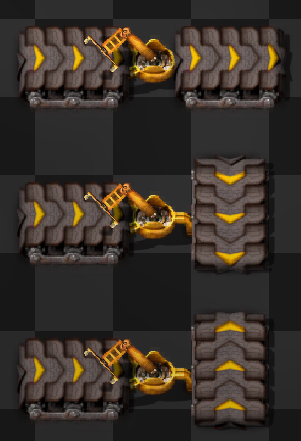
\includegraphics[width=\textwidth]{Figures//captures_joc/redundant_inserter.png}
        \caption{Combinacions redundants cinta-inseridor}
    \end{subfigure}
    \hfill
    \begin{subfigure}{0.45\textwidth}
        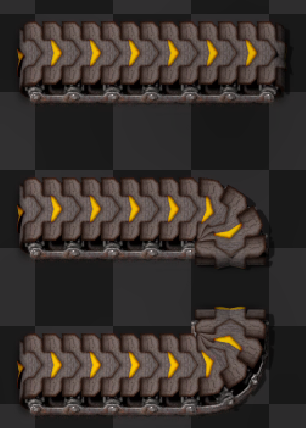
\includegraphics[width=\textwidth]{Figures//captures_joc/conveyor_alternative.png}
        \caption{Alternativa vàlida només amb cintes}
    \end{subfigure}
    \caption{Casos on un inseridor és redundant i pot ser substituït per una cinta obtenint el mateix resultat}
    \label{fig:redundant_inserter}
\end{figure}

Els casos on la cinta no apunta a l'inseridor els hem de permetre, ja que es tracten de bifurcacions a les rutes i són completament vàlides. De la mateixa manera si la cinta apunta a l'inseridor per la sortida d'aquest és un assemblador també s'ha de permetre, ja que una cinta per si sola no pot afegir objectes a un assemblador.\\

La restricció que implementa aquesta millora és força senzilla:

\begin{lstlisting}[language=Python, caption=Evitar inserdiors redundants]
for each cell (i, j) in the grid of size (height x width):
    prevent = []
    for each dir in [north, east, south, west]:
        in_x = i + displacement[dir][0]
        in_y = j + displacement[dir][1]
        out_x = i + displacement[opposite_dir[dir]][0]
        out_y = j + displacement[opposite_dir[dir]][1]
        if 0 <= in_x < height and 0 <= in_y < width and 0 <= out_x < height and 0 <= out_y < width:
        prevent.append(Implies(
                        And(inserter[i][j] == opposite_dir[dir],
                            inserter[i][j] == conveyor[in_x][in_y]),
                        conveyor[out_x][out_y] == empty))
    assert Implies(inserter[i][j] != empty, And(prevent))
\end{lstlisting}

El que es fa és, per cada casella \lstinline{(i, j)}, i per cada possible direcció, s'agafen les caselles d'entrada i sortida relatives a la direcció i la posició (\lstinline{in_x, in_y, out_x, out_y}), si el valor de la variable \lstinline{inserter[i][j]} és igual a la direcció oposada que estem mirant, és a dir la casella d'entrada, i la casella d'entrada és una cinta amb direcció igual a l'inseridor (cas que es vol detectar), llavors a la casella de sortida de l'inseridor no hi pot haver una cinta, sigui quina sigui la seva direcció, d'aquesta mare prevenim les combinacions redundants entre cintes i inseridors.

\begin{figure}[H]
    \centering
    \begin{subfigure}{0.45\textwidth}
        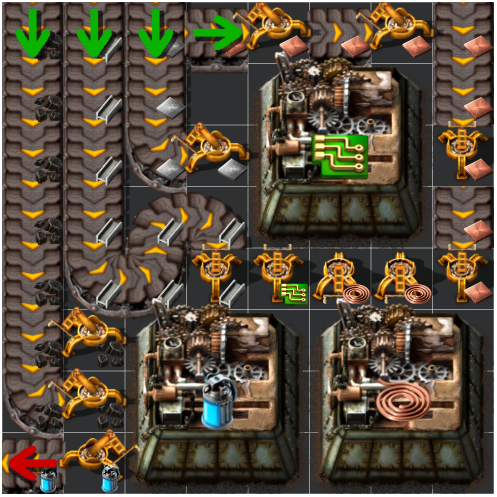
\includegraphics[width=\textwidth]{Figures//captures_joc/exemples_model/instancia_amb_redundancia.PNG}
        \caption{Sense aplicar la restricció}
    \end{subfigure}
    \hfill
    \begin{subfigure}{0.45\textwidth}
        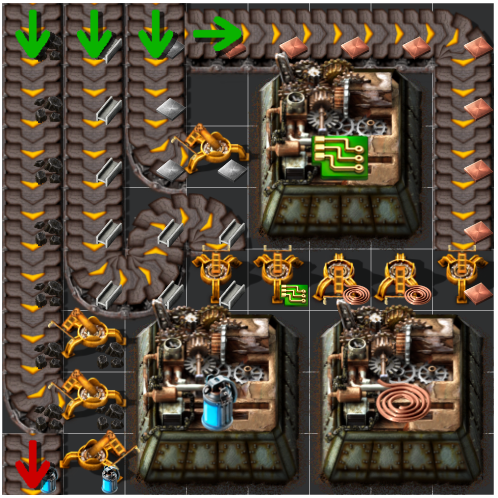
\includegraphics[width=\textwidth]{Figures//captures_joc/exemples_model/instancia_sense_redundancia.PNG}
        \caption{Aplicant la restricció}
    \end{subfigure}
    \caption{Comparació de la mateixa instància sense i aplicant la millora}
\end{figure}

\section{Criteris d'optimització}
Al model s'han incorporat tres criteris d'optimització diferents. N'hi ha un que és el bàsic i sempre es té en compte que és el que maximitza el nombre d'objectes produïts. Aquest criteri se li pot sumar l'optimització addicional que redueix el nombre d'elements que formen part d'una ruta i l'optimització que redueix la pèrdua d'objectes.\\
Tot seguit s'expliquen en detall els criteris d'optimització i les seves implementacions.

\subsection{Maximitzar la quantitat d'objectes}
Per poder maximitzar la quantitat d'objectes que surten del blueprint, cal poder identificar les variables \lstinline{item_flow_rate} a les posicions de sortida del blueprint. Això ho podem fer de manera molt senzilla, ja que les posicions de sortida del blueprint tracten d'un dels inputs del model. A partir d'aquí, només cal maximitzar la suma d'objectes a les posicions de sortida. Això s'ha fet de la següent manera:
\begin{lstlisting}[language=Python, caption=Quantitat d'objectes de sortida]
    def item_output(self):
        item_output = []
        for pos in output:
            i = pos[0]
            j = pos[1]
            item_output.append(output_flow_rate[i][j])
        return sum(item_output)
\end{lstlisting}

La implementació és molt senzilla, ja que el model es guarda en una llista de llistes \lstinline{output} les coordenades al blueprint de cada casella de sortida, així que iterant per aquestes coordenades i fent el sumatori de la variable \lstinline{item_flow_rate} a les posicions corresponents, només cal dir-li a l'optimitzador de Z3 que maximitzi aquest sumatori:

\begin{lstlisting}[language=Python, caption=Maximitzar el criteri, label=code:opt_flow]
    opt = Optimize()
    opt.maximize(item_flow_rate_behaviour.item_output())
\end{lstlisting}
La funció que retorna el sumatori es troba en una classe en forma de mètode que conté tota la logica del \lstinline{item_flow_rate} i es pot cridar amb el codi \ref{code:opt_flow}.

\subsection{Minimitzar la mida de les rutes}
De manera similar a l'anterior optimització, es necessita quantificar quants elements que formen part d'una ruta s'estan usant en una solució. Com s'ha explicat els elements que formen part d'una ruta són les cintes i els inseridors els quals en cas de ser usats tindran un valor a la variable \lstinline{route} més gran que 0. Així que per saber quants s'estan fent servir cal iterar per la variable \lstinline{route} i comptar quantes d'aquestes variables tenen un valor diferent de 0, indicant així que estan essent usades. El codi per fer aquest és molt simple:
\begin{lstlisting}[language=Python, caption=Quantitat d'elements de ruta]
    def route_length(self):
        return sum([If(self.route[i][j] == 0, 0, 1) for i in range(self.height) for j in range(self.width)])
\end{lstlisting}
El que s'està fent és usar un if-then-else que en cas que la variable \lstinline{route} sigui 0 llavors es torna 0 i en cas contrari 1, aquests valors se sumen i l'objectiu és minimitzar el sumatori, fent que el nombre d'assignacions iguals a 0 de la variable \lstinline{route} sigui el màxim possible, minimitzant així l'ús d'elements de ruta.
\begin{lstlisting}[language=Python, caption=Minimitzar el criteri]
    opt = Optimize()
    opt.minimize(route_behaviour.route_length())
\end{lstlisting}
El criteri d'optimització es pot minimitzar amb un \lstinline{Optimize()} de Z3, usant el mètode implementat a la classe \lstinline{route_behaviour} que n'implementa el mètode.

\subsection{Minimitzar la pèrdua d'objectes}
Finalment, com la resta de criteris d'optimització, s'ha d'establir que significa dins les variables del model la pèrdua d'objectes i quantificar-ho amb codi Z3.\\
Al context del problema del blueprint, la pèrdua d'objectes s'entén com a objectes dins la xarxa de cintes que no acaben essent usats pels assembladors, això es produeix quan l'última cinta d'una ruta acumula objectes.\\
A la figura \ref{fig:item_loss_example} es poden veure les cintes que poden acumular objectes i ens interessa minimitzar el seu valor a la variable \lstinline{output_flow_rate}. Aquestes cintes concretament són sempre les que apunten a un inseridor amb la mateixa direcció que la cinta.
\begin{figure}[H]
    \centering
    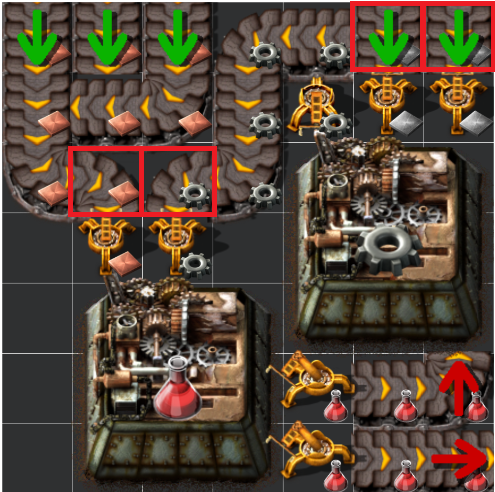
\includegraphics[width=0.5\linewidth]{Figures/captures_joc/exemples_model/item_loss_example.png}
    \caption{Caselles on es poden acumular objectes a les cintes en forma de pèrdua}
    \label{fig:item_loss_example}
\end{figure}
La implementació per quantificar el valor d'\lstinline{output_flow_rate} d'aquestes cintes és el següent:

\begin{lstlisting}[language=Python, caption=Quantitat de pèrdua d'objectes]
    def item_loss(self):
        loss = []
        for each dir in [north, east, south, west]:
            x = i + displacement[dir][0]
            y = j + displacement[dir][1]
            if 0 <= x < height and 0 <= y < width:
                loss+=If(And(conveyor[i][j] != empty, inserter[x][y] == conveyor[i][j]), output_flow_rate[i][j], 0)
        return sum(loss)
\end{lstlisting}

El que es fa és, per cada cinta, es miren les caselles veïnes dins el blueprint i si la casella veïna de la cinta és un inseridor amb la mateixa direcció, és suma el seu valor de la variable \lstinline{output_flow_rate}.\\

\begin{lstlisting}[language=Python, caption=Minimitzar el criteri]
    opt = Optimize()
    opt.minimize(item_flow_rate_behaviour.item_loss())
\end{lstlisting}

La crida per minimitzar és la mateixa que l'anterior optimització, però la funció a optimitzar es troba implementada a la classe \lstinline{item_flow_rate_behaviour}.

